\section{Графики решения}
1. По теореме Виета $x_1+x_2=-\cfrac{a+3}{3},\ x_1x_2=\cfrac{a}{3}.$ Тогда $\cfrac{1}{x_1}+\cfrac{1}{x_2}=\cfrac{x_1+x_2}{x_1x_2}=
\cfrac{-\cfrac{a+3}{3}}{\cfrac{a}{3}}=-\cfrac{a+3}{a}=2,\ 2a=-a-3,\ a=-1.$ Параболу $y=3x^2+2x-1$ построим по трём точкам $(-1;0),\ \left(\cfrac{1}{3};0\right)$ и\\$ \left(-\cfrac{1}{3};-\cfrac{4}{3}\right).$
$$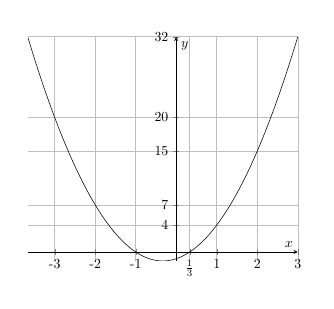
\begin{tikzpicture}[scale=0.5]
\begin{axis}[
    axis lines = middle,
    grid=major,
    legend pos={south west},
    xlabel = {$x$},
    ylabel = {$y$},
    xtick={-4, -3, -2, -1,0.333, 1,2, 3},
    xticklabels={-4,-3, -2, -1,$\frac{1}{3}$, 1,2,3},
    ytick={-5,20,7,4, 15,32},
              ]
	\addplot[domain=-3.66:3, samples=100, color=black] {3*x*x+2*x-1};
%\addplot[domain=-3.1:2.5, samples=100, color=red] {70*abs(1-2*abs(abs(x)-2))-10*x^2+10*x-70};
	%\addlegendentry{$\text{Рис. 1}$};
\end{axis}
\end{tikzpicture}$$
2. По теореме Виета $x_1+x_2=\cfrac{1-a}{3},\ x_1x_2=\cfrac{a}{3}.$ Тогда $\cfrac{1}{x_1}+\cfrac{1}{x_2}=\cfrac{x_1+x_2}{x_1x_2}=
\cfrac{\cfrac{1-a}{3}}{\cfrac{a}{3}}=\cfrac{1-a}{a}=-2,\ -2a=1-a,\ a=-1.$ Параболу $y=3x^2-2x-1$ построим по трём точкам $(1;0),\ \left(-\cfrac{1}{3};0\right)$ и\\$ \left(\cfrac{1}{3};-\cfrac{4}{3}\right).$
$$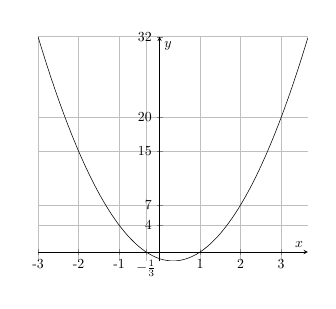
\begin{tikzpicture}[scale=0.5]
\begin{axis}[
    axis lines = middle,
    grid=major,
    legend pos={south west},
    xlabel = {$x$},
    %xlabel style={below right},
    ylabel = {$y$},
    xtick={-3, -2, -1,-0.333, 1,2, 3},
    xticklabels={-3, -2, -1,$-\frac{1}{3}$, 1,2,3},
    ytick={-5,20,7,4, 15,32},
               ]
	\addplot[domain=-3:3.66, samples=100, color=black] {3*x*x-2*x-1};
%\addplot[domain=-3.1:2.5, samples=100, color=red] {70*abs(1-2*abs(abs(x)-2))-10*x^2+10*x-70};
	%\addlegendentry{$\text{Рис. 1}$};
\end{axis}
\end{tikzpicture}$$
3. $y=\cfrac{x^2+3x}{|x+3|}+x=\begin{cases} 2x,\ x>-3,\\ 0,\ x<-3.\end{cases}$
$$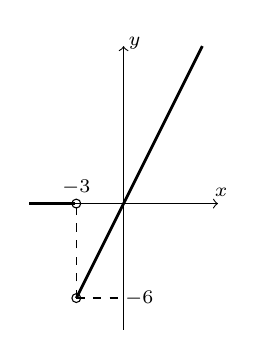
\begin{tikzpicture}[scale=0.2]
\tikzset {line01/.style={line width =0.5pt}}
\tikzset{line02/.style={line width =1pt}}
\tikzset{line03/.style={dashed,line width =0.5pt}}
%\filldraw [black] (0,0) circle (1pt);
\draw [->] (-6,0) -- (6,0);
\draw [->] (0,-8) -- (0,10);
\draw[line02] (-6,0) -- (-3.1,0);
\draw[line02] (-3,-6) -- (5,10);
\draw[line03] (-3,-6) -- (-3,0);
\draw[line03] (-3,-6) -- (0,-6);
\draw (6.2,0.7) node {\scriptsize $x$};
\draw (-3,1) node {\scriptsize $-3$};
\draw (1,-6) node {\scriptsize $-6$};
%\draw (-0.7,3) node {\scriptsize $3$};
\draw (0.7,10.2) node {\scriptsize $y$};
\draw (-3,0) circle (8pt);
\draw (-3,-6) circle (8pt);
\end{tikzpicture}$$
4. $y=\cfrac{2x-x^2}{|x-2|}+x=\begin{cases} 0,\ x>2,\\ 2x,\ x<2.\end{cases}$
$$\begin{tikzpicture}[scale=0.2]
\tikzset {line01/.style={line width =0.5pt}}
\tikzset{line02/.style={line width =1pt}}
\tikzset{line03/.style={dashed,line width =0.5pt}}
%\filldraw [black] (0,0) circle (1pt);
\draw [->] (-6,0) -- (6,0);
\draw [->] (0,-8) -- (0,10);
\draw[line02] (2.1,0) -- (6,0);
\draw[line02] (-3,-6) -- (2,4);
\draw[line03] (2,0) -- (2,4);
\draw[line03] (0,4) -- (2,4);
\draw (6.2,0.7) node {\scriptsize $x$};
\draw (2,-1) node {\scriptsize $2$};
\draw (-1,4) node {\scriptsize $4$};
%\draw (-0.7,3) node {\scriptsize $3$};
\draw (0.7,10.2) node {\scriptsize $y$};
\draw (2,0) circle (8pt);
\draw (2,4) circle (8pt);
\end{tikzpicture}$$
5. По теореме Виета $x_1+x_2=15,\ x_1x_2=q.$ Тогда $\cfrac{1}{x_1}+\cfrac{1}{x_2}=\cfrac{x_1+x_2}{x_1x_2}=\cfrac{15}{q}=\cfrac{5}{12}\Rightarrow q=36.$ Построим параболу $x^2-15x+36$ по трём точкам $(4;0),\ (12;0),\ \left(\cfrac{15}{2}, -\cfrac{81}{4}\right).$
$$ 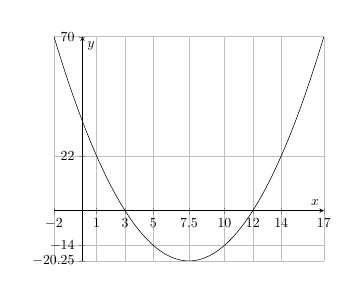
\begin{tikzpicture}[scale=0.5]
\begin{axis}[
    axis lines = middle,
    grid=major,
    legend pos={south west},
    xlabel = {$x$},
    ylabel = {$y$},
    %ymin=-80,
    %ymax=250,
    xtick={-2, 1, 3, 5, 7.5, 10, 12, 14, 17},
    ytick={70,22,-14,-20.25,-30}          ]
	\addplot[domain=-2:17, samples=100, color=black] {x*x-15*x+36};
%\addplot[domain=-3.1:2.5, samples=100, color=red] {70*abs(1-2*abs(abs(x)-2))-10*x^2+10*x-70};
	%\addlegendentry{$\text{Рис. 1}$};
\end{axis}
\end{tikzpicture}$$
6. По теореме Виета $x_1+x_2=-9,\ x_1x_2=q.$ Тогда $\cfrac{1}{x_1}+\cfrac{1}{x_2}=\cfrac{x_1+x_2}{x_1x_2}=\cfrac{-9}{q}=-\cfrac{1}{2}\Rightarrow q=18.$ Построим параболу $x^2+9x+18$ по трём точкам $(-3;0),\ (-6;0),\ \left(-\cfrac{9}{2}, -\cfrac{9}{4}\right).$
$$\begin{tikzpicture}[scale=0.5]
\begin{axis}[
    axis lines = middle,
    grid=major,
    legend pos={south west},
    xlabel = {$x$},
    ylabel = {$y$},
    %ymin=-80,
    %ymax=250,
    xtick={-10, -7, -6, -4.5, -3, 1},
    xticklabels={-10,-7, -6, $-\cfrac{9}{2}$, -3, 1},
    ytick={28,4,-2.25},
    yticklabels={28,4,$-\cfrac{9}{4}$}             ]
	\addplot[domain=-10:1, samples=100, color=black] {x*x+9*x+18};
%\addplot[domain=-3.1:2.5, samples=100, color=red] {70*abs(1-2*abs(abs(x)-2))-10*x^2+10*x-70};
	%\addlegendentry{$\text{Рис. 1}$};
\end{axis}
\end{tikzpicture}$$
7. $y=\cfrac{|x+1|}{x+1}(x-1)=\begin{cases} x-1,\ x>-1,\\ 1-x,\ x<-1.\end{cases}$
$$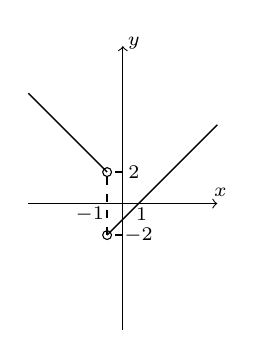
\begin{tikzpicture}[scale=0.2]
\tikzset {line01/.style={line width =0.5pt}}
\tikzset{line02/.style={line width =1pt}}
\tikzset{line03/.style={dashed,line width =0.5pt}}
%\filldraw [black] (0,0) circle (1pt);
\draw [->] (-6,0) -- (6,0);
\draw [->] (0,-8) -- (0,10);
\draw[line01] (-6,7) -- (-1,2);
\draw[line01] (-1,-2) -- (6,5);
\draw[line03] (-1,-2) -- (-1,2);
\draw[line03] (0,2) -- (-1,2);
\draw[line03] (0,-2) -- (-1,-2);
\draw (6.2,0.7) node {\scriptsize $x$};
\draw (1,-2) node {\scriptsize $-2$};
\draw (0.7,2) node {\scriptsize $2$};
\draw (1.2,-0.7) node {\scriptsize $1$};
\draw (-2.1,-0.7) node {\scriptsize $-1$};
\draw (0.7,10.2) node {\scriptsize $y$};
\draw (-1,2) circle (8pt);
\draw (-1,-2) circle (8pt);
\end{tikzpicture}$$
8. $y=\cfrac{|x-1|}{x-1}(x+1)=\begin{cases} x+1,\ x>1,\\ -x-1,\ x<1.\end{cases}$
$$\begin{tikzpicture}[scale=0.2]
\tikzset {line01/.style={line width =0.5pt}}
\tikzset{line02/.style={line width =1pt}}
\tikzset{line03/.style={dashed,line width =0.5pt}}
%\filldraw [black] (0,0) circle (1pt);
\draw [->] (-6,0) -- (6,0);
\draw [->] (0,-8) -- (0,10);
\draw[line01] (-6,5) -- (1,-2);
\draw[line01] (1,2) -- (6,7);
\draw[line03] (1,-2) -- (1,2);
\draw[line03] (0,2) -- (1,2);
\draw[line03] (0,-2) -- (1,-2);
\draw (6.2,0.7) node {\scriptsize $x$};
\draw (-1.2,-2) node {\scriptsize $-2$};
\draw (-0.7,2) node {\scriptsize $2$};
\draw (1.4,-0.7) node {\scriptsize $1$};
\draw (-2.1,-0.7) node {\scriptsize $-1$};
\draw (0.7,10.2) node {\scriptsize $y$};
\draw (1,2) circle (8pt);
\draw (1,-2) circle (8pt);
\end{tikzpicture}$$
9. По теореме Виета $x_1+x_2=8,\ x_1x_2=q.$ Тогда $x_1^2+x_2^2=(x_1+x_2)^2-2x_1x_2=64-2q=34,\ q=15.$ Параболу $x^2-8x+15$ построим по трём точкам $(3;0),\ (5;0),\ (4;-1).$
$$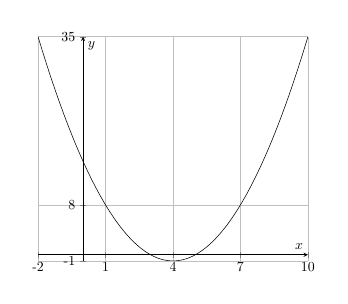
\begin{tikzpicture}[scale=0.5]
\begin{axis}[
    axis lines = middle,
    grid=major,
    legend pos={south west},
    xlabel = {$x$},
    ylabel = {$y$},
    %ymin=-80,
    %ymax=250,
    xtick={-2, 1, 4, 7, 10},
    xticklabels={-2, 1, 4, 7, 10},
    ytick={-1,8,35},
    yticklabels={-1,8,35}             ]
	\addplot[domain=-2:10, samples=100, color=black] {x*x-8*x+15};
%\addplot[domain=-3.1:2.5, samples=100, color=red] {70*abs(1-2*abs(abs(x)-2))-10*x^2+10*x-70};
	%\addlegendentry{$\text{Рис. 1}$};
\end{axis}
\end{tikzpicture}$$
10. По теореме Виета $x_1+x_2=8,\ x_1x_2=q.$ Тогда $(x_1-x_2)^2=(x_1+x_2)^2-4x_1x_2=64-4q=4,\ q=15.$ Параболу $x^2-8x+15$ построим по трём точкам $(3;0),\ (5;0),\ (4;-1).$
$$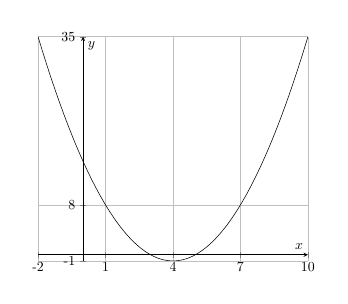
\begin{tikzpicture}[scale=0.5]
\begin{axis}[
    axis lines = middle,
    grid=major,
    legend pos={south west},
    xlabel = {$x$},
    ylabel = {$y$},
    %ymin=-80,
    %ymax=250,
    xtick={-2, 1, 4, 7, 10},
    xticklabels={-2, 1, 4, 7, 10},
    ytick={-1,8,35},
    yticklabels={-1,8,35}             ]
	\addplot[domain=-2:10, samples=100, color=black] {x*x-8*x+15};
%\addplot[domain=-3.1:2.5, samples=100, color=red] {70*abs(1-2*abs(abs(x)-2))-10*x^2+10*x-70};
	%\addlegendentry{$\text{Рис. 1}$};
\end{axis}
\end{tikzpicture}$$
11. $y=\cfrac{x^2+2x+1}{|x+1|}=\cfrac{|x+1|^2}{|x+1|}=|x+1|,\ x\neq-1.$
$$\begin{tikzpicture}[scale=0.2]
\tikzset {line01/.style={line width =0.5pt}}
\tikzset{line02/.style={line width =1pt}}
\tikzset{line03/.style={dashed,line width =0.5pt}}
%\filldraw [black] (0,0) circle (1pt);
\draw [->] (-6,0) -- (6,0);
\draw [->] (0,-8) -- (0,10);
\draw[line01] (-6,5) -- (-1,0);
\draw[line01] (4,5) -- (-1,0);
%\draw[line03] (1,-2) -- (1,2);
%\draw[line03] (0,2) -- (1,2);
%\draw[line03] (0,-2) -- (1,-2);
\draw (6.2,0.7) node {\scriptsize $x$};
%\draw (-1.2,-2) node {\scriptsize $-2$};
%\draw (-0.7,2) node {\scriptsize $2$};
\draw (0.7,1) node {\scriptsize $1$};
\draw (-1,-0.7) node {\scriptsize $-1$};
\draw (0.7,10.2) node {\scriptsize $y$};
\draw (-1,0) circle (8pt);
%\draw (1,-2) circle (8pt);
\end{tikzpicture}$$
12. $y=\cfrac{x^2-2x+1}{|x-1|}=\cfrac{|x-1|^2}{|x-1|}=|x-1|,\ x\neq1.$
$$\begin{tikzpicture}[scale=0.2]
\tikzset {line01/.style={line width =0.5pt}}
\tikzset{line02/.style={line width =1pt}}
\tikzset{line03/.style={dashed,line width =0.5pt}}
%\filldraw [black] (0,0) circle (1pt);
\draw [->] (-6,0) -- (6,0);
\draw [->] (0,-8) -- (0,10);
\draw[line01] (-6,7) -- (1,0);
\draw[line01] (8,7) -- (1,0);
%\draw[line03] (1,-2) -- (1,2);
%\draw[line03] (0,2) -- (1,2);
%\draw[line03] (0,-2) -- (1,-2);
\draw (6.2,0.7) node {\scriptsize $x$};
%\draw (-1.2,-2) node {\scriptsize $-2$};
%\draw (-0.7,2) node {\scriptsize $2$};
\draw (-0.7,1) node {\scriptsize $1$};
\draw (1,-0.9) node {\scriptsize $1$};
\draw (0.7,10.2) node {\scriptsize $y$};
\draw (1,0) circle (8pt);
%\draw (1,-2) circle (8pt);
\end{tikzpicture}$$
13. $y=\cfrac{2x^2-5x+2}{x-2}\cdot(x+1)=\cfrac{(2x-1)(x-2)}{x-2}\cdot(x+1)=2x^2+x-1,\ x\neq2.$ Построим параболу по трём точкам $(-1;0),\ \left(\cfrac{1}{2};0\right),\ \left(-\cfrac{1}{4};-\cfrac{9}{8}\right).$
$$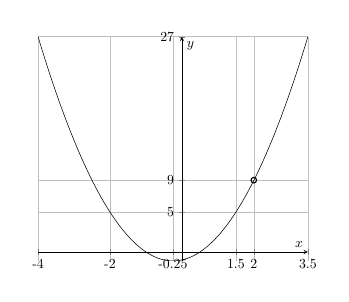
\begin{tikzpicture}[scale=0.5]
\begin{axis}[
    axis lines = middle,
    grid=major,
    legend pos={south west},
    xlabel = {$x$},
    ylabel = {$y$},
    %ymin=-80,
    %ymax=250,
    xtick={-4, -2, -0.25, 1.5,2, 3.5},
    xticklabels={-4, -2, -0.25, 1.5,2, 3.5},
    ytick={27,5,9},
    yticklabels={27,5,9}             ]
	\addplot[domain=-4:3.5, samples=100, color=black] {(2*x-1)*(x+1)};
%\addplot[domain=-3.1:2.5, samples=100, color=red] {70*abs(1-2*abs(abs(x)-2))-10*x^2+10*x-70};
	%\addlegendentry{$\text{Рис. 1}$};
\end{axis}
\draw (5.48,2.05) circle (2pt);
\end{tikzpicture}$$
14. $y=\cfrac{2x^2+5x+2}{x+2}\cdot(x-1)=\cfrac{(2x+1)(x+2)}{x+2}\cdot(x-1)=2x^2-x-1,\ x\neq-2.$ Построим параболу по трём точкам $(1;0),\ \left(-\cfrac{1}{2};0\right),\ \left(\cfrac{1}{4};-\cfrac{9}{8}\right).$
$$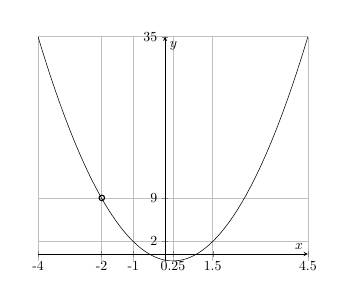
\begin{tikzpicture}[scale=0.5]
\begin{axis}[
    axis lines = middle,
    grid=major,
    legend pos={south west},
    xlabel = {$x$},
    ylabel = {$y$},
    %ymin=-80,
    %ymax=250,
    xtick={-4, -2, -1, 0.25, 1.5, 4.5},
    xticklabels={-4, -2, -1, 0.25, 1.5, 4.5},
    ytick={35,9,2},
    yticklabels={35,9,2}             ]
	\addplot[domain=-4:4.5, samples=100, color=black] {(2*x+1)*(x-1)};
%\addplot[domain=-3.1:2.5, samples=100, color=red] {70*abs(1-2*abs(abs(x)-2))-10*x^2+10*x-70};
	%\addlegendentry{$\text{Рис. 1}$};
\end{axis}
\draw (1.62,1.6) circle (2pt);
\end{tikzpicture}$$
15. $y=\cfrac{x^2-5x+6}{|x-2|}=\cfrac{(x-2)(x-3)}{|x-2|}=\begin{cases} x-3,\ x>2,\\ 3-x,\ x<2.\end{cases}$
$$\begin{tikzpicture}[scale=0.2]
\tikzset {line01/.style={line width =0.5pt}}
\tikzset{line02/.style={line width =1pt}}
\tikzset{line03/.style={dashed,line width =0.5pt}}
%\filldraw [black] (0,0) circle (1pt);
\draw [->] (-6,0) -- (6,0);
\draw [->] (0,-8) -- (0,10);
\draw[line01] (-6,9) -- (2,1);
\draw[line01] (2,-1) -- (6,3);
\draw[line03] (2,-1) -- (2,1);
\draw[line03] (0,1) -- (2,1);
\draw[line03] (0,-1) -- (2,-1);
\draw (6.2,0.7) node {\scriptsize $x$};
\draw (-1.2,-1) node {\scriptsize $-1$};
\draw (-0.7,1) node {\scriptsize $1$};
\draw (-0.7,3) node {\tiny $3$};
\draw (1.4,-0.5) node {\tiny $2$};
\draw (3.2,-0.7) node {\tiny $3$};
\draw (0.7,10.2) node {\scriptsize $y$};
\draw (2,-1) circle (8pt);
\draw (2,1) circle (8pt);
\end{tikzpicture}$$
16. $y=\cfrac{x^2+5x+6}{|x+2|}=\cfrac{(x+2)(x+3)}{|x+2|}=\begin{cases} x+3,\ x>-2,\\ -x-3,\ x<-2.\end{cases}$
$$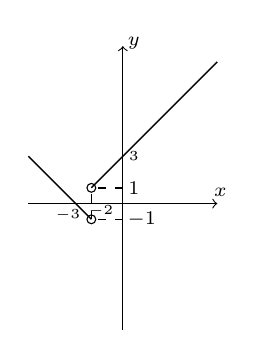
\begin{tikzpicture}[scale=0.2]
\tikzset {line01/.style={line width =0.5pt}}
\tikzset{line02/.style={line width =1pt}}
\tikzset{line03/.style={dashed,line width =0.5pt}}
%\filldraw [black] (0,0) circle (1pt);
\draw [->] (-6,0) -- (6,0);
\draw [->] (0,-8) -- (0,10);
\draw[line01] (-6,3) -- (-2,-1);
\draw[line01] (-2,1) -- (6,9);
\draw[line03] (-2,-1) -- (-2,1);
\draw[line03] (0,1) -- (-2,1);
\draw[line03] (0,-1) -- (-2,-1);
\draw (6.2,0.7) node {\scriptsize $x$};
\draw (1.2,-1) node {\scriptsize $-1$};
\draw (0.7,1) node {\scriptsize $1$};
\draw (0.7,3) node {\tiny $3$};
\draw (-1.4,-0.5) node {\tiny $-2$};
\draw (-3.5,-0.7) node {\tiny $-3$};
\draw (0.7,10.2) node {\scriptsize $y$};
\draw (-2,-1) circle (8pt);
\draw (-2,1) circle (8pt);
\end{tikzpicture}$$
17. $(y-2x)\left(|x|-5-y\right)=0\Leftrightarrow\left[\begin{array}{l}y-2x=0,\\ |x|=y+5.\end{array}\right.\Leftrightarrow
\left[\begin{array}{l}y=2x,\\ \begin{cases}\left[\begin{array}{l}x=y+5,\\ x=-y-5.\end{array}\right.\\ y+5\geqslant0\end{cases}\end{array}\right.\Leftrightarrow
\left[\begin{array}{l}y=2x,\\ \begin{cases}\left[\begin{array}{l}y=x-5,\\ y=-x-5.\end{array}\right.\\ y\geqslant-5\end{cases}\end{array}\right.$
$$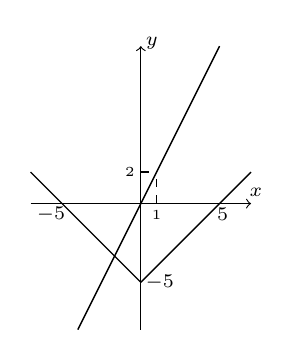
\begin{tikzpicture}[scale=0.2]
\tikzset {line01/.style={line width =0.5pt}}
\tikzset{line02/.style={line width =1pt}}
\tikzset{line03/.style={dashed,line width =0.5pt}}
%\filldraw [black] (0,0) circle (1pt);
\draw [->] (-7,0) -- (7,0);
\draw [->] (0,-8) -- (0,10);
\draw[line01] (-4,-8) -- (5,10);
\draw[line01] (7,2) -- (0,-5);
\draw[line01] (-7,2) -- (0,-5);
%\draw[line03] (-2,-1) -- (-2,1);
\draw[line03] (0,2) -- (1,2);
\draw[line03] (1,0) -- (1,2);
\draw (7.3,0.7) node {\scriptsize $x$};
\draw (1.2,-5) node {\scriptsize $-5$};
\draw (5.2,-0.7) node {\scriptsize $5$};
\draw (-5.7,-0.7) node {\scriptsize $-5$};
\draw (1,-0.7) node {\tiny $1$};
\draw (-0.7,2) node {\tiny $2$};
%\draw (-1.4,-0.5) node {\tiny $-2$};
%\draw (-3.5,-0.7) node {\tiny $-3$};
\draw (0.7,10.2) node {\scriptsize $y$};
%\draw (-2,-1) circle (8pt);
%\draw (-2,1) circle (8pt);
\end{tikzpicture}$$
18. $f(x)=\cfrac{\sqrt{1+\left(\cfrac{x^2-1}{2x}\right)^2}}{(x^2+1)\cdot\cfrac{1}{x}}=
\cfrac{x\sqrt{\cfrac{x^4+2x^2+1}{4x^2}}}{x^2+1}=\cfrac{x\left|\cfrac{x^2+1}{2x}\right|}{x^2+1}=\cfrac{x}{2|x|}=\begin{cases}\cfrac{1}{2},\ x>0,\\ -\cfrac{1}{2},\ x<0.\end{cases}$
$$\begin{tikzpicture}[scale=0.2]
\tikzset {line01/.style={line width =0.5pt}}
\tikzset{line02/.style={line width =1pt}}
\tikzset{line03/.style={dashed,line width =0.5pt}}
%\filldraw [black] (0,0) circle (1pt);
\draw [->] (-7,0) -- (7,0);
\draw [->] (0,-8) -- (0,10);
\draw[line01] (0,2) -- (7,2);
\draw[line01] (-7,-2) -- (0,-2);
%\draw[line01] (-7,2) -- (0,-5);
%\draw[line03] (-2,-1) -- (-2,1);
%\draw[line03] (0,2) -- (1,2);
%\draw[line03] (1,0) -- (1,2);
\draw (7.3,0.7) node {\scriptsize $x$};
%\draw (1.2,-5) node {\scriptsize $-5$};
%\draw (5.2,-0.7) node {\scriptsize $5$};
%\draw (-5.7,-0.7) node {\scriptsize $-5$};
\draw (-1.2,2) node {\tiny $\cfrac{1}{2}$};
\draw (1.5,-2) node {\tiny $-\cfrac{1}{2}$};
%\draw (-1.4,-0.5) node {\tiny $-2$};
%\draw (-3.5,-0.7) node {\tiny $-3$};
\draw (0.7,10.2) node {\scriptsize $y$};
\draw (0,-2) circle (8pt);
\draw (0,2) circle (8pt);
\end{tikzpicture}$$
19. По теореме Виета $x_1+x_2=\cfrac{a}{2},\ x_1x_2=-\cfrac{a}{2}.$ Тогда $\cfrac{x_1}{x_2}+\cfrac{x_2}{x_1}=\cfrac{x_1^2+x_2^2}{x_1x_2}=\cfrac{(x_1+x_2)^2-2x_1x_2}{x_1x_2}=\cfrac{\cfrac{a^2}{4}+a}{-\cfrac{a}{2}}=-\cfrac{a+4}{2}=-3,5\Rightarrow a=3.$ Построим параболу $y=2x^2-3x-3$ по трём точкам \\ $(-2;11),\ \left(\cfrac{7}{2};11\right),\ \left(\cfrac{3}{4};-\cfrac{33}{8}\right).$
$$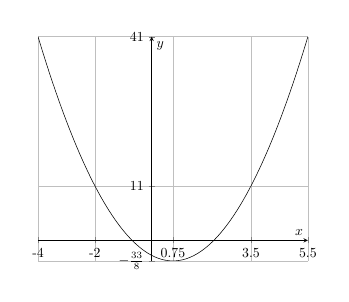
\begin{tikzpicture}[scale=0.5]
\begin{axis}[
    axis lines = middle,
    grid=major,
    legend pos={south west},
    xlabel = {$x$},
    ylabel = {$y$},
    %ymin=-80,
    %ymax=250,
    xtick={-4, -2, 0.75, 3.5, 5.5},
    xticklabels={-4, -2, 0.75, 3.5, 5.5},
    ytick={41,11,-4.125},
    yticklabels={41,11,$-\frac{33}{8}$}             ]
	\addplot[domain=-4:5.5, samples=100, color=black] {2*x*x-3*x-3};
%\addplot[domain=-3.1:2.5, samples=100, color=red] {70*abs(1-2*abs(abs(x)-2))-10*x^2+10*x-70};
	%\addlegendentry{$\text{Рис. 1}$};
\end{axis}
\end{tikzpicture}$$
20. $|y|=x+1\Leftrightarrow \begin{cases}\left[\begin{array}{l}y=x+1,\\ y=-x-1.\end{array}\right.\\  x\geqslant-1\end{cases}$
$$\begin{tikzpicture}[scale=0.2]
\tikzset {line01/.style={line width =0.5pt}}
\tikzset{line02/.style={line width =1pt}}
\tikzset{line03/.style={dashed,line width =0.5pt}}
%\filldraw [black] (0,0) circle (1pt);
\draw [->] (-7,0) -- (7,0);
\draw [->] (0,-8) -- (0,10);
\draw[line01] (-1,0) -- (7,-8);
\draw[line01] (-1,0) -- (7,8);
%\draw[line01] (-7,2) -- (0,-5);
%\draw[line03] (-2,-1) -- (-2,1);
%\draw[line03] (0,2) -- (1,2);
%\draw[line03] (1,0) -- (1,2);
\draw (7.3,0.7) node {\scriptsize $x$};
%\draw (1.2,-5) node {\scriptsize $-5$};
%\draw (5.2,-0.7) node {\scriptsize $5$};
%\draw (-5.7,-0.7) node {\scriptsize $-5$};
%\draw (-1.2,2) node {\tiny $\cfrac{1}{2}$};
%\draw (1.5,-2) node {\tiny $-\cfrac{1}{2}$};
\draw (0.7,1) node {\tiny $1$};
\draw (1.3,-1) node {\tiny $-1$};
\draw (-1.1,-1) node {\tiny $-1$};
%\draw (-3.5,-0.7) node {\tiny $-3$};
\draw (0.7,10.2) node {\scriptsize $y$};
\end{tikzpicture}$$
21. $|y|=x-1\Leftrightarrow \begin{cases}\left[\begin{array}{l}y=x-1,\\ y=1-x.\end{array}\right.\\  x\geqslant1\end{cases}$
$$\begin{tikzpicture}[scale=0.2]
\tikzset {line01/.style={line width =0.5pt}}
\tikzset{line02/.style={line width =1pt}}
\tikzset{line03/.style={dashed,line width =0.5pt}}
%\filldraw [black] (0,0) circle (1pt);
\draw [->] (-7,0) -- (7,0);
\draw [->] (0,-8) -- (0,10);
\draw[line01] (1,0) -- (7,6);
\draw[line01] (1,0) -- (7,-6);
%\draw[line01] (-7,2) -- (0,-5);
%\draw[line03] (-2,-1) -- (-2,1);
%\draw[line03] (0,2) -- (1,2);
%\draw[line03] (1,0) -- (1,2);
\draw (7.3,0.7) node {\scriptsize $x$};
%\draw (1.2,-5) node {\scriptsize $-5$};
%\draw (5.2,-0.7) node {\scriptsize $5$};
%\draw (-5.7,-0.7) node {\scriptsize $-5$};
%\draw (-1.2,2) node {\tiny $\cfrac{1}{2}$};
%\draw (1.5,-2) node {\tiny $-\cfrac{1}{2}$};
%\draw (0.7,1) node {\tiny $1$};
\draw (1.1,-1) node {\tiny $1$};
%\draw (-1.1,-1) node {\tiny $-1$};
%\draw (-3.5,-0.7) node {\tiny $-3$};
\draw (0.7,10.2) node {\scriptsize $y$};
\end{tikzpicture}$$
22. $y=|x|+|x+2|=\begin{cases} 2x+2,\ x>0,\\ 2,\ x\in[-2;0],\\ -2x-2,\ x<-2.\end{cases}$
$$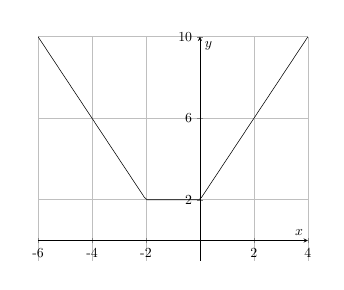
\begin{tikzpicture}[scale=0.5]
\begin{axis}[
    axis lines = middle,
    grid=major,
    legend pos={south west},
    xlabel = {$x$},
    ylabel = {$y$},
    ymin=-1,
    %ymax=250,
    xtick={-6, -4, -2, 2,4},
    xticklabels={-6, -4, -2, 2,4},
    ytick={-2, 6, 2, 10},
    yticklabels={-2, 6, 2, 10}             ]
	\addplot[domain=-6:4, samples=100, color=black] {abs(x)+abs(x+2)};
%\addplot[domain=-3.1:2.5, samples=100, color=red] {70*abs(1-2*abs(abs(x)-2))-10*x^2+10*x-70};
	%\addlegendentry{$\text{Рис. 1}$};
\end{axis}
\end{tikzpicture}$$
23. $y=|x|+|x-2|=\begin{cases} 2x-2,\ x>2,\\ 2,\ x\in[0;2],\\ -2x+2,\ x<0.\end{cases}$
$$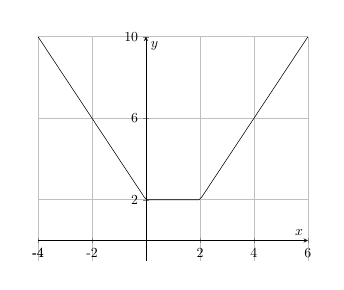
\begin{tikzpicture}[scale=0.5]
\begin{axis}[
    axis lines = middle,
    grid=major,
    legend pos={south west},
    xlabel = {$x$},
    ylabel = {$y$},
    ymin=-1,
    %ymax=250,
    xtick={-4, -4, -2, 2,4,6},
    xticklabels={-4, -4, -2, 2,4,6},
    ytick={-2, 6, 2, 10},
    yticklabels={-2, 6, 2, 10}             ]
	\addplot[domain=-4:6, samples=100, color=black] {abs(x)+abs(x-2)};
%\addplot[domain=-3.1:2.5, samples=100, color=red] {70*abs(1-2*abs(abs(x)-2))-10*x^2+10*x-70};
	%\addlegendentry{$\text{Рис. 1}$};
\end{axis}
\end{tikzpicture}$$
24. Прямая может пересекать ось ординат в точке $(0;2)$ или $(0;-2).$ Пусть прямая имеет уравнение $y=ax+b.$ Тогда в первом случае $\begin{cases}a+b=2,\\ b=2.\end{cases}\Leftrightarrow y=2.$ Во втором случае $\begin{cases}a+b=2,\\ b=-2.\end{cases}\Leftrightarrow y=4x-2.$\\
25. Прямая может пересекать ось ординат в точке $(0;2)$ или $(0;-2).$ Пусть прямая имеет уравнение $y=ax+b.$ Тогда в первом случае $\begin{cases}-a+b=2,\\ b=2.\end{cases}\Leftrightarrow y=2.$ Во втором случае $\begin{cases}-a+b=2,\\ b=-2.\end{cases}\Leftrightarrow y=-4x-2.$\\
26. $y=\cfrac{x^3-2x^2-5x+6}{x+2}=\cfrac{x^2(x+2)-4x(x+2)+3(x+2)}{x+2}=\cfrac{(x+2)(x^2-4x+3)}{x+2}=x^2-4x+3,$\\$ x\neq-2.$ Построим параболу по трём точкам $(1;0),\ (3;0),\ (2;-1).$
$$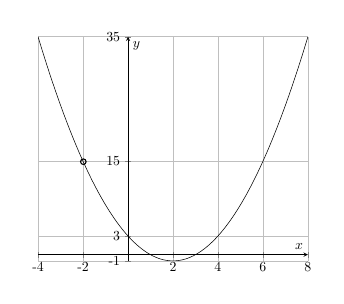
\begin{tikzpicture}[scale=0.5]
\begin{axis}[
    axis lines = middle,
    grid=major,
    legend pos={south west},
    xlabel = {$x$},
    ylabel = {$y$},
    ymin=-1,
    %ymax=250,
    xtick={-4, -2, 2,4,6,8},
    xticklabels={-4,-2, 2,4,6,8},
    ytick={35, 15, -1, 3},
    yticklabels={35, 15, -1, 3}            ]
	\addplot[domain=-4:8, samples=100, color=black] {x*x-4*x+3};
%\addplot[domain=-3.1:2.5, samples=100, color=red] {70*abs(1-2*abs(abs(x)-2))-10*x^2+10*x-70};
	%\addlegendentry{$\text{Рис. 1}$};
\end{axis}
\draw (1.15,2.52) circle (2pt);
\end{tikzpicture}$$
27. $y=\cfrac{x^3+2x^2-5x-6}{x-2}=\cfrac{x^2(x-2)+4x(x-2)+3(x-2)}{x-2}=\cfrac{(x-2)(x^2+4x+3)}{x-2}=x^2+4x+3,$\\$ x\neq2.$ Построим параболу по трём точкам $(-1;0),\ (-3;0),\ (-2;-1).$
$$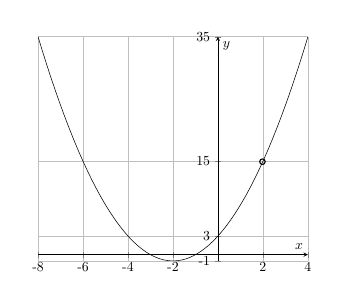
\begin{tikzpicture}[scale=0.5]
\begin{axis}[
    axis lines = middle,
    grid=major,
    legend pos={south west},
    xlabel = {$x$},
    ylabel = {$y$},
    ymin=-1,
    %ymax=250,
    xtick={4, 2, -2,-4,-6,-8},
    xticklabels={4, 2, -2,-4,-6,-8},
    ytick={35, 15, -1, 3},
    yticklabels={35, 15, -1, 3}            ]
	\addplot[domain=-8:4, samples=100, color=black] {x*x+4*x+3};
%\addplot[domain=-3.1:2.5, samples=100, color=red] {70*abs(1-2*abs(abs(x)-2))-10*x^2+10*x-70};
	%\addlegendentry{$\text{Рис. 1}$};
\end{axis}
\draw (5.7,2.52) circle (2pt);
\end{tikzpicture}$$
28. $y=\cfrac{x^2-3x+2}{|x-2|}=\cfrac{(x-2)(x-1)}{|x-2|}=\begin{cases} x-1,\ x>2,\\ 1-x,\ x<2.\end{cases}.$
$$\begin{tikzpicture}[scale=0.2]
\tikzset {line01/.style={line width =0.5pt}}
\tikzset{line02/.style={line width =1pt}}
\tikzset{line03/.style={dashed,line width =0.5pt}}
%\filldraw [black] (0,0) circle (1pt);
\draw [->] (-6,0) -- (6,0);
\draw [->] (0,-8) -- (0,10);
\draw[line01] (-6,7) -- (2,-1);
\draw[line01] (2,1) -- (6,5);
\draw[line03] (2,-1) -- (2,1);
\draw[line03] (0,1) -- (2,1);
\draw[line03] (0,-1) -- (2,-1);
\draw (6.2,0.7) node {\scriptsize $x$};
\draw (-1.2,-1) node {\scriptsize $-1$};
\draw (-0.7,1) node {\scriptsize $1$};
%\draw (-0.7,3) node {\tiny $3$};
\draw (2.6,-0.5) node {\tiny $2$};
%\draw (3.2,-0.7) node {\tiny $3$};
\draw (0.7,10.2) node {\scriptsize $y$};
\draw (2,-1) circle (8pt);
\draw (2,1) circle (8pt);
\end{tikzpicture}$$
29. $y=\cfrac{x^2-4x+3}{|x-3|}=\cfrac{(x-3)(x-1)}{|x-3|}=\begin{cases} x-1,\ x>3,\\ 1-x,\ x<3.\end{cases}.$
$$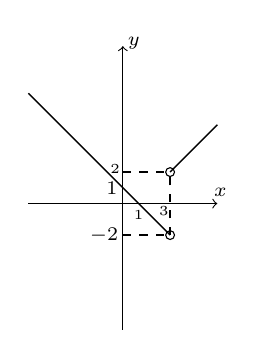
\begin{tikzpicture}[scale=0.2]
\tikzset {line01/.style={line width =0.5pt}}
\tikzset{line02/.style={line width =1pt}}
\tikzset{line03/.style={dashed,line width =0.5pt}}
%\filldraw [black] (0,0) circle (1pt);
\draw [->] (-6,0) -- (6,0);
\draw [->] (0,-8) -- (0,10);
\draw[line01] (-6,7) -- (3,-2);
\draw[line01] (3,2) -- (6,5);
\draw[line03] (3,-2) -- (3,2);
\draw[line03] (0,2) -- (3,2);
\draw[line03] (0,-2) -- (3,-2);
\draw (6.2,0.7) node {\scriptsize $x$};
\draw (-1.2,-2) node {\scriptsize $-2$};
\draw (-0.7,1) node {\scriptsize $1$};
\draw (-0.5,2.2) node {\tiny $2$};
\draw (1,-0.7) node {\tiny $1$};
%\draw (-0.7,3) node {\tiny $3$};
\draw (2.6,-0.5) node {\tiny $3$};
%\draw (3.2,-0.7) node {\tiny $3$};
\draw (0.7,10.2) node {\scriptsize $y$};
\draw (3,-2) circle (8pt);
\draw (3,2) circle (8pt);
\end{tikzpicture}$$
30. Пусть прямая задаётся уравнением $y=3x+b,$ тогда $3\cdot1+b=2,\ b=-1,$ прямая имеет вид $y=3x-1.$\\
31. Пусть прямая задаётся уравнением $y=3x+b,$ тогда $3\cdot2+b=4,\ b=-2,$ прямая имеет вид $y=3x-2.$\\
32. $y=1-|x-2|=\begin{cases} 1-x+2=3-x,\ x\geqslant2,\\ 1+x-2=x-1,\ x<2.\end{cases}$
$$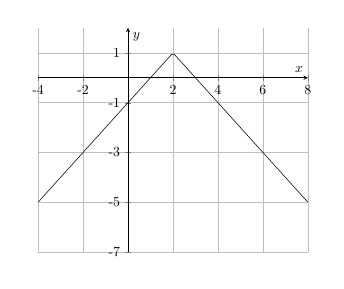
\begin{tikzpicture}[scale=0.5]
\begin{axis}[
    axis lines = middle,
    grid=major,
    legend pos={south west},
    xlabel = {$x$},
    ylabel = {$y$},
    ymin=-7,
    ymax=2,
    xtick={ -4, -2, 2,4,6,8},
    xticklabels={ -4, -2, 2,4,6,8},
    ytick={-7,-5,-3, 1, -1},
    yticklabels={-7,-5,-3, 1, -1}            ]
	\addplot[domain=-4:8, samples=100, color=black] {1-abs(x-2)};
%\addplot[domain=-3.1:2.5, samples=100, color=red] {70*abs(1-2*abs(abs(x)-2))-10*x^2+10*x-70};
	%\addlegendentry{$\text{Рис. 1}$};
\end{axis}
\end{tikzpicture}$$
33. $y=1-|x+2|=\begin{cases} 1-x-2=-1-x,\ x\geqslant-2,\\ 1+x+2=x+3,\ x<-2.\end{cases}$
$$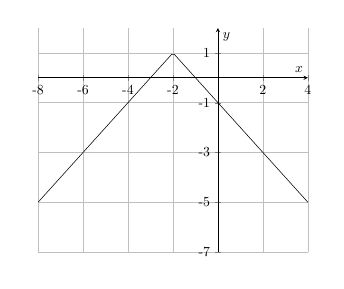
\begin{tikzpicture}[scale=0.5]
\begin{axis}[
    axis lines = middle,
    grid=major,
    legend pos={south west},
    xlabel = {$x$},
    ylabel = {$y$},
    ymin=-7,
    ymax=2,
    xtick={ 4, 2, -2,-4,-6,-8},
    xticklabels={ 4, 2, -2,-4,-6,-8},
    ytick={-7,-5,-3, 1, -1},
    yticklabels={-7,-5,-3, 1, -1}            ]
	\addplot[domain=-8:4, samples=100, color=black] {1-abs(x+2)};
%\addplot[domain=-3.1:2.5, samples=100, color=red] {70*abs(1-2*abs(abs(x)-2))-10*x^2+10*x-70};
	%\addlegendentry{$\text{Рис. 1}$};
\end{axis}
\end{tikzpicture}$$
34. Пусть прямая задана уравнением $y=kx+b,$ тогда она отсекает на осях координат отрезки, имеющие длины $|b|$ и $\left|\cfrac{b}{k}\right|.$ Тогда
$|b|=\left|\cfrac{b}{k}\right|\Leftrightarrow |b|\left(1-\cfrac{1}{|k|}\right)=0\Leftrightarrow
\left[\begin{array}{l}b=0,\\ k=1,\\ k=-1.\end{array}\right.$ Если $b=0,$ то прямая не отсекает отрезков от осей координат. При $k=1$ имеем равенство $2+b=3,\ b=1.$
При $k=-1$ имеем равенство $-2+b=3,\ b=5.$ Таким образом, уравнение прямой может иметь вид $y=x+1$ или $y=5-x.$\\
35. Пусть прямая задана уравнением $y=kx+b,$ тогда она отсекает на осях координат отрезки, имеющие длины $|b|$ и $\left|\cfrac{b}{k}\right|.$ Тогда
$|b|=\left|\cfrac{b}{k}\right|\Leftrightarrow |b|\left(1-\cfrac{1}{|k|}\right)=0\Leftrightarrow
\left[\begin{array}{l}b=0,\\ k=1,\\ k=-1.\end{array}\right.$ Если $b=0,$ то прямая не отсекает отрезков от осей координат. При $k=1$ имеем равенство $3+b=2,\ b=-1.$
При $k=-1$ имеем равенство $-3+b=2,\ b=5.$ Таким образом, уравнение прямой может иметь вид $y=x-1$ или $y=5-x.$\\
36. $y=\cfrac{x^2-x-20}{x-5}=\cfrac{(x-5)(x+4)}{x-5}=x+4,\ x\neq5.$
$$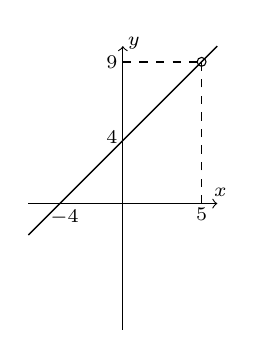
\begin{tikzpicture}[scale=0.2]
\tikzset {line01/.style={line width =0.5pt}}
\tikzset{line02/.style={line width =1pt}}
\tikzset{line03/.style={dashed,line width =0.5pt}}
%\filldraw [black] (0,0) circle (1pt);
\draw [->] (-6,0) -- (6,0);
\draw [->] (0,-8) -- (0,10);
\draw[line01] (-6,-2) -- (6,10);
\draw[line03] (5,0) -- (5,9);
\draw[line03] (0,9) -- (5,9);
%\draw[line03] (0,-2) -- (1,-2);
\draw (6.2,0.7) node {\scriptsize $x$};
%\draw (-1.2,-2) node {\scriptsize $-2$};
%\draw (-0.7,2) node {\scriptsize $2$};
\draw (-0.7,4.2) node {\scriptsize $4$};
\draw (-0.7,9) node {\scriptsize $9$};
\draw (5,-0.7) node {\scriptsize $5$};
\draw (-3.7,-0.9) node {\scriptsize $-4$};
\draw (0.7,10.2) node {\scriptsize $y$};
%\draw (1,0) circle (8pt);
\draw (5,9) circle (8pt);
\end{tikzpicture}$$
37. $y=\cfrac{x^2-x-2}{x-2}=\cfrac{(x-2)(x+1)}{x-2}=x+1,\ x\neq2.$
$$\begin{tikzpicture}[scale=0.2]
\tikzset {line01/.style={line width =0.5pt}}
\tikzset{line02/.style={line width =1pt}}
\tikzset{line03/.style={dashed,line width =0.5pt}}
%\filldraw [black] (0,0) circle (1pt);
\draw [->] (-6,0) -- (6,0);
\draw [->] (0,-8) -- (0,10);
\draw[line01] (-6,-5) -- (6,7);
\draw[line03] (2,0) -- (2,3);
\draw[line03] (0,3) -- (2,3);
%\draw[line03] (0,-2) -- (1,-2);
\draw (6.2,0.7) node {\scriptsize $x$};
%\draw (-1.2,-2) node {\scriptsize $-2$};
%\draw (-0.7,2) node {\scriptsize $2$};
\draw (-0.7,1.2) node {\scriptsize $1$};
\draw (-0.7,3) node {\scriptsize $3$};
\draw (2,-0.7) node {\scriptsize $2$};
\draw (-0.8,-0.9) node {\tiny $-1$};
\draw (0.7,10.2) node {\scriptsize $y$};
%\draw (1,0) circle (8pt);
\draw (2,3) circle (8pt);
\end{tikzpicture}$$
38. $y=\cfrac{(x+1)(x-3)}{|x-1|+2}=\begin{cases} \cfrac{(x+1)(x-3)}{x-1+2},\ x\geqslant1,\\ \cfrac{(x+1)(x-3)}{1-x+2},\ x<1.\end{cases}=
\begin{cases} x-3,\ x\geqslant1,\\ -x-1,\ x<1.\end{cases}$
$$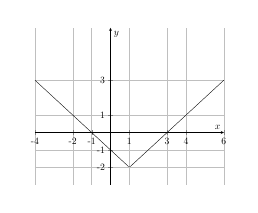
\begin{tikzpicture}[scale=0.35]
\begin{axis}[
    axis lines = middle,
    grid=major,
    legend pos={south west},
    xlabel = {$x$},
    ylabel = {$y$},
    ymin=-3,
    ymax=6,
    xtick={ -4, -1, 1, 4,3, 6,-2},
    xticklabels={ -4, -1, 1, 4,3, 6,-2},
    ytick={ -2, 1, -1,3},
    yticklabels={ -2, 1, -1,3}            ]
	\addplot[domain=-4:6, samples=100, color=black] {(x+1)*(x-3)/(abs(x-1)+2)};
%\addplot[domain=-3.1:2.5, samples=100, color=red] {70*abs(1-2*abs(abs(x)-2))-10*x^2+10*x-70};
	%\addlegendentry{$\text{Рис. 1}$};
\end{axis}
\end{tikzpicture}$$
39. $y=\cfrac{(x-1)(x-3)}{|x-2|+1}=\begin{cases} \cfrac{(x-1)(x-3)}{x-2+1},\ x\geqslant2,\\ \cfrac{(x-1)(x-3)}{2-x+1},\ x<2.\end{cases}=
\begin{cases} x-3,\ x\geqslant2,\\ 1-x,\ x<2.\end{cases}$
$$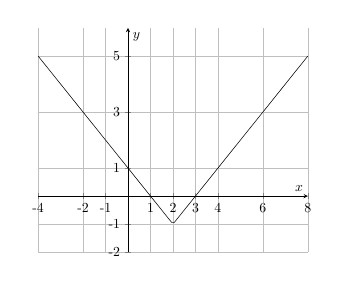
\begin{tikzpicture}[scale=0.5]
\begin{axis}[
    axis lines = middle,
    grid=major,
    legend pos={south west},
    xlabel = {$x$},
    ylabel = {$y$},
    ymin=-2,
    ymax=6,
    xtick={ -4, -1, 1, 4,3, 6,-2,2,8},
    xticklabels={ -4, -1, 1, 4,3, 6,-2,2,8},
    ytick={ -2, 1, -1,3,5},
    yticklabels={ -2, 1, -1,3,5}            ]
	\addplot[domain=-4:8, samples=100, color=black] {(x-1)*(x-3)/(abs(x-2)+1)};
%\addplot[domain=-3.1:2.5, samples=100, color=red] {70*abs(1-2*abs(abs(x)-2))-10*x^2+10*x-70};
	%\addlegendentry{$\text{Рис. 1}$};
\end{axis}
\end{tikzpicture}$$
40. Один из катетов этого треугольника равен 2, значит другой должен быть равен $4\cdot2:2=4.$ Тогда эта прямая может проходить через точку $(4;0)$ или $(-4;0).$ В обоих случаях $b=2$ (так как прямая проходит через точку $(0;2).)$ Пусть прямая задана уравнением $y=kx+b.$ В первом случае $4k+2=0,\ k=-\cfrac{1}{2},$ а во втором --- $-4k+2=0,\ k=\cfrac{1}{2}.$ Значит, прямая может иметь уравнение $y=2-\frac{1}{2}x$ или $y=2+\frac{1}{2}x.$\\
41. Один из катетов этого треугольника равен 3, значит другой должен быть равен $9\cdot2:3=6.$ Тогда эта прямая может проходить через точку $(6;0)$ или $(-6;0).$ В обоих случаях $b=3$ (так как прямая проходит через точку $(0;3).)$ Пусть прямая задана уравнением $y=kx+b.$ В первом случае $6k+3=0,\ k=-\cfrac{1}{2},$ а во втором --- $-6k+3=0,\ k=\cfrac{1}{2}.$ Значит, прямая может иметь уравнение $y=3-\frac{1}{2}x$ или $y=3+\frac{1}{2}x.$\\
42. $|y|=|x-2|\Leftrightarrow \left[\begin{array}{l}y=x-2,\\ y=2-x.\end{array}\right.$
$$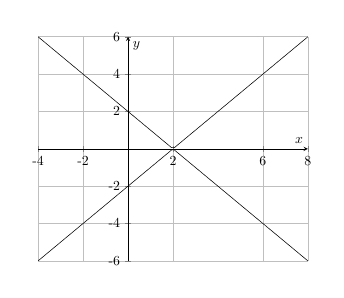
\begin{tikzpicture}[scale=0.5]
\begin{axis}[
    axis lines = middle,
    grid=major,
    legend pos={south west},
    xlabel = {$x$},
    ylabel = {$y$},
    ymin=-6,
    ymax=6,
    xtick={-4,-2,2,6,8},
    xticklabels={-4,-2,2,6,8},
    ytick={ 6, 4,-6, -4, 2, -2},
    yticklabels={ 6, 4,-6, -4, 2, -2}            ]
	\addplot[domain=-4:8, samples=100, color=black] {abs(x-2)};
\addplot[domain=-4:8, samples=100, color=black] {-abs(x-2)};
%\addplot[domain=-3.1:2.5, samples=100, color=red] {70*abs(1-2*abs(abs(x)-2))-10*x^2+10*x-70};
	%\addlegendentry{$\text{Рис. 1}$};
\end{axis}
\end{tikzpicture}$$
43. $|y|=|x-1|\Leftrightarrow \left[\begin{array}{l}y=x-1,\\ y=1-x.\end{array}\right.$
$$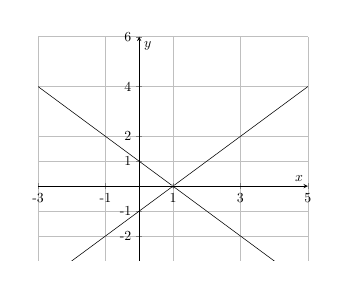
\begin{tikzpicture}[scale=0.5]
\begin{axis}[
    axis lines = middle,
    grid=major,
    legend pos={south west},
    xlabel = {$x$},
    ylabel = {$y$},
    ymin=-3,
    ymax=6,
    xtick={-3,-1,1,3,5},
    xticklabels={-3,-1,1,3,5},
    ytick={ 6, 2,-6, -2,1,-1,4,-4},
    yticklabels={ 6, 2,-6, -2,1,-1,4,-4}           ]
	\addplot[domain=-3:5, samples=100, color=black] {abs(x-1)};
\addplot[domain=-3:5, samples=100, color=black] {-abs(x-1)};
%\addplot[domain=-3.1:2.5, samples=100, color=red] {70*abs(1-2*abs(abs(x)-2))-10*x^2+10*x-70};
	%\addlegendentry{$\text{Рис. 1}$};
\end{axis}
\end{tikzpicture}$$
44. Чтобы $k$ сократилось, необходимо взять $x=1,$ тогда $y-2=0,\ y=2,$ то есть точка имеет координаты $(1;2).$\\
45. Чтобы $k$ сократилось, необходимо взять $x=-1,$ тогда $y+2=0,\ y=-2,$ то есть точка имеет координаты $(-1;-2).$\\
46. Пусть парабола задана уравнением $y=ax^2+bx+c.$ Раз её вершина находится в начале координат, $-\cfrac{b}{2a}=0\Rightarrow b=0,\ 0+0+c=0\Rightarrow c=0.$ Раз парабола проходит через точку $A,$ имеем соотношение $a\cot(-1)^2=0,75\Rightarrow a=0,75$ и парабола задана уравнением $y=0,75x^2.$ Найдём точки пересечения с прямой $y=12:\ 0,75x^2=12,\ x^2=16,\ x=\pm4.$ Значит, они пересекаются в точках $(-4;12)$ и $(4;12).$\\
47. $y=|x-2|+|x+1|=\left[\begin{array}{l}x-2+x+1=2x-1,\ x>2,\\ 2-x+x+1=3,\ x\in[-1;2],\\ -x+2-x-1=-2x+1,\ x<-1.\end{array}\right.$
$$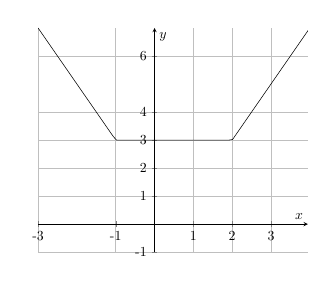
\begin{tikzpicture}[scale=0.5]
\begin{axis}[
    axis lines = middle,
    grid=major,
    legend pos={south west},
    xlabel = {$x$},
    ylabel = {$y$},
    ymin=-1,
    ymax=7,
    xtick={-3,-1,1,3,5,2},
    xticklabels={-3,-1,1,3,5,2},
    ytick={ 6, 2,-6, -2,1,-1,4,-4,3},
    yticklabels={ 6, 2,-6, -2,1,-1,4,-4,3}           ]
	\addplot[domain=-3:5, samples=100, color=black] {abs(x-2)+abs(x+1)};
%\addplot[domain=-3:5, samples=100, color=black] {-abs(x-1)};
%\addplot[domain=-3.1:2.5, samples=100, color=red] {70*abs(1-2*abs(abs(x)-2))-10*x^2+10*x-70};
	%\addlegendentry{$\text{Рис. 1}$};
\end{axis}
\end{tikzpicture}$$
48. Прямая может пересекать ось абсцисс в точке $(3;0)$ или $(-3;0).$ Пусть прямая имеет уравнение $y=kx+b.$ Тогда в первом случае $\begin{cases}2a+b=1,\\ 3a+b=0.\end{cases}\Leftrightarrow y=3-x.$ Во втором случае $\begin{cases}2a+b=1,\\ -3a+b=0.\end{cases}\Leftrightarrow y=\frac{1}{5}x+\frac{3}{5}.$\\
49. $y=\sqrt{1-4x+4x^2}-3=|2x-1|-3=\begin{cases}2x-1-3=2x-4,\ x\geqslant\cfrac{1}{2},\\ -2x+1-3=-2x-2,\ x<\cfrac{1}{2}.\end{cases}$
$$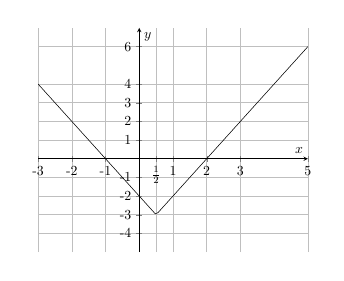
\begin{tikzpicture}[scale=0.5]
\begin{axis}[
    axis lines = middle,
    grid=major,
    legend pos={south west},
    xlabel = {$x$},
    ylabel = {$y$},
    ymin=-5,
    ymax=7,
    xtick={-3,-1,1,3,5,2,-2,0.5},
    xticklabels={-3,-1,1,3,5,2,-2,$\frac{1}{2}$},
    ytick={ 6, 2,-6, -2,1,-1,4,-4,3,-3},
    yticklabels={ 6, 2,-6, -2,1,-1,4,-4,3,-3}           ]
	\addplot[domain=-3:5, samples=100, color=black] {abs(1-2*x)-3};
%\addplot[domain=-3:5, samples=100, color=black] {-abs(x-1)};
%\addplot[domain=-3.1:2.5, samples=100, color=red] {70*abs(1-2*abs(abs(x)-2))-10*x^2+10*x-70};
	%\addlegendentry{$\text{Рис. 1}$};
\end{axis}
\end{tikzpicture}$$
50. $y=\sqrt{1+4x+4x^2}-3=|2x+1|-3=\begin{cases}2x+1-3=2x-2,\ x\geqslant-\cfrac{1}{2},\\ -2x-1-3=-2x-4,\ x<-\cfrac{1}{2}.\end{cases}$
$$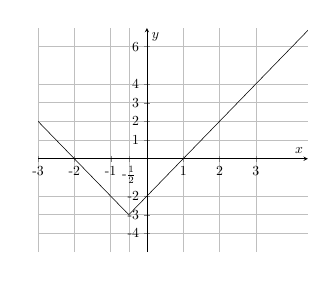
\begin{tikzpicture}[scale=0.5]
\begin{axis}[
    axis lines = middle,
    grid=major,
    legend pos={south west},
    xlabel = {$x$},
    ylabel = {$y$},
    ymin=-5,
    ymax=7,
    xtick={-3,-1,1,3,5,2,-2,-0.5},
    xticklabels={-3,-1,1,3,5,2,-2,-$\frac{1}{2}$},
    ytick={ 6, 2,-6, -2,1,4,-4,3,-3},
    yticklabels={ 6, 2,-6, -2,1,4,-4,3,-3}           ]
	\addplot[domain=-3:5, samples=100, color=black] {abs(1+2*x)-3};
%\addplot[domain=-3:5, samples=100, color=black] {-abs(x-1)};
%\addplot[domain=-3.1:2.5, samples=100, color=red] {70*abs(1-2*abs(abs(x)-2))-10*x^2+10*x-70};
	%\addlegendentry{$\text{Рис. 1}$};
\end{axis}
\end{tikzpicture}$$
51. Приравняем прямую к параболе: $kx=(x-1)^2,\ x^2-2x+1-kx=0,\ x^2-(k+2)x+1=0.$ Это уравнение имеет единственное решение при $D=(k+2)^2-4=0,\ k(k+4)=0,\ k=0$ или $k=-4.$\\
52. Приравняем прямую к параболе: $kx=(x+1)^2,\ x^2+2x+1-kx=0,\ x^2-(k-2)x+1=0.$ Это уравнение имеет единственное решение при $D=(k-2)^2-4=0,\ k(k-4)=0,\ k=0$ или $k=4.$\\
53. Пусть прямая задана уравнением $y=kx+b,$ тогда $\begin{cases} k+b=3,\\ 3k+b=7.\end{cases}\Leftrightarrow
\begin{cases} k+b=3,\\ 2k=4.\end{cases}\Leftrightarrow\begin{cases} k=2,\\ b=1.\end{cases}$\\$\Rightarrow y=2x+1.$\\
54. Пусть прямая задана уравнением $y=kx+b,$ тогда $\begin{cases} 2k+b=5,\\ 4k+b=9.\end{cases}\Leftrightarrow
\begin{cases} 2k+b=5,\\ 2k=4.\end{cases}\Leftrightarrow$\\$\begin{cases} k=2,\\ b=1.\end{cases}\Rightarrow y=2x+1.$\\
55. $\cfrac{(x^2-4)(y-x+1)}{x-2}=0\Leftrightarrow\begin{cases} \left[\begin{array}{l}x=2,\\ x=-2,\\ y=x-1.\end{array}\right.\\ x\neq2.\end{cases}$
$$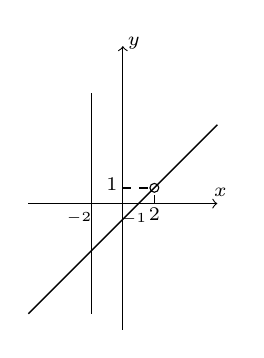
\begin{tikzpicture}[scale=0.2]
\tikzset {line01/.style={line width =0.5pt}}
\tikzset{line02/.style={line width =1pt}}
\tikzset{line03/.style={dashed,line width =0.5pt}}
%\filldraw [black] (0,0) circle (1pt);
\draw [->] (-6,0) -- (6,0);
\draw [->] (0,-8) -- (0,10);
\draw[line01] (-6,-7) -- (6,5);
\draw[line01] (-2,-7) -- (-2,7);
\draw[line03] (2,0) -- (2,1);
\draw[line03] (0,1) -- (2,1);
%\draw[line03] (0,-2) -- (1,-2);
\draw (6.2,0.7) node {\scriptsize $x$};
%\draw (-1.2,-2) node {\scriptsize $-2$};
%\draw (-0.7,2) node {\scriptsize $2$};
\draw (-0.7,1.2) node {\scriptsize $1$};
\draw (0.7,-1) node {\tiny $-1$};
\draw (2,-0.7) node {\scriptsize $2$};
\draw (-2.8,-0.9) node {\tiny $-2$};
\draw (0.7,10.2) node {\scriptsize $y$};
\draw (2,1) circle (8pt);
%\draw (-2,-3) circle (8pt);
\end{tikzpicture}$$
56. $\cfrac{(x^2-9)(y-x+1)}{x-3}=0\Leftrightarrow\begin{cases} \left[\begin{array}{l}x=3,\\ x=-3,\\ y=x-1.\end{array}\right.\\ x\neq3.\end{cases}$
$$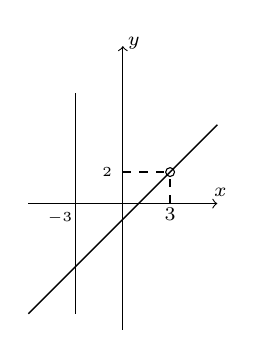
\begin{tikzpicture}[scale=0.2]
\tikzset {line01/.style={line width =0.5pt}}
\tikzset{line02/.style={line width =1pt}}
\tikzset{line03/.style={dashed,line width =0.5pt}}
%\filldraw [black] (0,0) circle (1pt);
\draw [->] (-6,0) -- (6,0);
\draw [->] (0,-8) -- (0,10);
\draw[line01] (-6,-7) -- (6,5);
\draw[line01] (-3,-7) -- (-3,7);
\draw[line03] (3,0) -- (3,2);
\draw[line03] (0,2) -- (3,2);
%\draw[line03] (0,-2) -- (1,-2);
\draw (6.2,0.7) node {\scriptsize $x$};
%\draw (-1.2,-2) node {\scriptsize $-2$};
%\draw (-0.7,2) node {\scriptsize $2$};
%\draw (-0.7,1.2) node {\scriptsize $1$};
\draw (-1,2) node {\tiny $2$};
\draw (3,-0.7) node {\scriptsize $3$};
\draw (-4,-0.9) node {\tiny $-3$};
\draw (0.7,10.2) node {\scriptsize $y$};
\draw (3,2) circle (8pt);
%\draw (-2,-3) circle (8pt);
\end{tikzpicture}$$
57. Приравняем прямую к параболе: $2x-3=(x-k)^2,\ x^2-2kx+k^2-2x+3=0,$\\$ x^2-2(k+1)x+k^2+3=0.$ У них есть общая точка, если это уравнение имеет хотя бы одно решение, то есть $D=4(k+1)^2-4(k^2+3)\geqslant0,\ k^2+2k+1-k^2-3\geqslant0,\ k\geqslant1.$\\
58. Приравняем прямую к параболе: $2x+3=(x-k)^2,\ x^2-2kx+k^2-2x-3=0,$\\$ x^2-2(k+1)x+k^2-3=0.$ У них есть общая точка, если это уравнение имеет хотя бы одно решение, то есть $D=4(k+1)^2-4(k^2-3)\geqslant0,\ k^2+2k+1-k^2+3\geqslant0,\ k\geqslant-2.$\\
59. Через точки $(0;3)$ и $(1;1)$ проходит только график на рисунке 1.\\
60. Через точки $(0;-2)$ и $(-1;1)$ проходит только график на рисунке 1.\\
61. $y=\cfrac{3x^2-8x+4}{|2x-2|-x}=\cfrac{(3x-2)(x-2)}{|2x-2|-x}=\begin{cases} \cfrac{(3x-2)(x-2)}{x-2}=3x-2,\ x\geqslant1,\ x\neq2,\\ \cfrac{(3x-2)(x-2)}{2-3x}=2-x,\ x<1,\ x\neq\cfrac{2}{3}.\end{cases}$
$$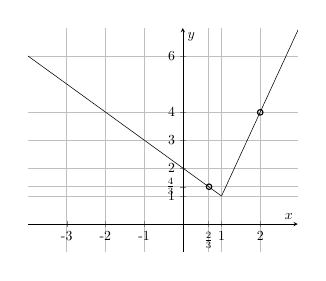
\begin{tikzpicture}[scale=0.5]
\begin{axis}[
    axis lines = middle,
    grid=major,
    legend pos={south west},
    xlabel = {$x$},
    ylabel = {$y$},
    ymin=-1,
    ymax=7,
    xtick={-3,-1,1,3,5,2,-2,0.666},
    xticklabels={-3,-1,1,3,5,2,-2,$\frac{2}{3}$},
    ytick={ 6, 2,-6, -2,1,4,-4,3,-3,1.333},
    yticklabels={ 6, 2,-6, -2,1,4,-4,3,-3,$\frac{4}{3}$}           ]
	\addplot[domain=1:6, samples=100, color=black] {3*x-2};
\addplot[domain=-4:1, samples=100, color=black] {2-x};
%\addplot[domain=-3.1:2.5, samples=100, color=red] {70*abs(1-2*abs(abs(x)-2))-10*x^2+10*x-70};
	%\addlegendentry{$\text{Рис. 1}$};
\end{axis}
\draw (4.6,1.66) circle (2pt);
\draw (5.9,3.55) circle (2pt);
\end{tikzpicture}$$
По графику определим, что прямая $y=a$ не имеет с графиком общих точек при $a<1.$\\
62. $y=\cfrac{3x^2+8x+4}{|2x+2|+x}=\cfrac{(3x+2)(x+2)}{|2x+2|+x}=\begin{cases} \cfrac{(3x+2)(x+2)}{3x+2}=x+2,\ x\geqslant-1,\ x\neq-\cfrac{2}{3},\\ \cfrac{(3x+2)(x+2)}{-x-2}=-3x-2,\ x<-1,\ x\neq-2.\end{cases}$
$$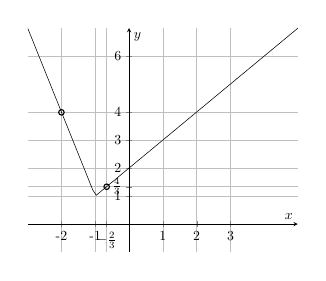
\begin{tikzpicture}[scale=0.5]
\begin{axis}[
    axis lines = middle,
    grid=major,
    legend pos={south west},
    xlabel = {$x$},
    ylabel = {$y$},
    ymin=-1,
    ymax=7,
    xtick={-3,-1,1,3,5,2,-2,-0.666},
    xticklabels={-3,-1,1,3,5,2,-2,$-\frac{2}{3}$},
    ytick={ 6, 2,-6, -2,1,4,-4,3,-3,1.333},
    yticklabels={ 6, 2,-6, -2,1,4,-4,3,-3,$\frac{4}{3}$}           ]
	\addplot[domain=-4:6, samples=100, color=black] {(3*x*x+8*x+4)/(abs(2*x+2)+x)};
%\addplot[domain=-4:1, samples=100, color=black] {2-x};
%\addplot[domain=-3.1:2.5, samples=100, color=red] {70*abs(1-2*abs(abs(x)-2))-10*x^2+10*x-70};
	%\addlegendentry{$\text{Рис. 1}$};
\end{axis}
\draw (2,1.66) circle (2pt);
\draw (0.85,3.55) circle (2pt);
\end{tikzpicture}$$
По графику определим, что прямая $y=a$ не имеет с графиком общих точек при $a<1.$\\
63. Найдём точки пересечения графика функции с осью абсцисс: $|2x-2|-1=0,\ |2x-2|=1,\ 2x-2=\pm1,\ x=\cfrac{3}{2}$ или $x=\cfrac{1}{2}.$ Она ограничивает с осью абсцисс треугольник с вершинами $(1;-1), \left(\cfrac{3}{2};0\right),\ \left(\cfrac{1}{2};0\right).$ Его основание имеет длину $\cfrac{3}{2}-\cfrac{1}{2}=1,$ как и высота, опущенная из вершины $(1;-1),$ а значит его площадь равна $\cfrac{1}{2}\cdot1\cdot1=\cfrac{1}{2}.$\\
64. Найдём точки пересечения графика функции с осью абсцисс: $|2x+2|-1=0,\ |2x+2|=1,\ 2x+2=\pm1,\ x=-\cfrac{3}{2}$ или $x=-\cfrac{1}{2}.$ Она ограничивает с осью абсцисс треугольник с вершинами $(-1;-1), \left(-\cfrac{3}{2};0\right),\ \left(-\cfrac{1}{2};0\right).$ Его основание имеет длину $\cfrac{3}{2}-\cfrac{1}{2}=1,$ как и высота, опущенная из вершины $(-1;-1),$ а значит его площадь равна $\cfrac{1}{2}\cdot1\cdot1=\cfrac{1}{2}.$\\
65. а) Первый график проходит через точку $(0;-72),$ значит он --- синий, а второй --- красный.\\
б) Исходя из графика, найдём ответ $x\in(-3;-2)\cup(1;2)\cup(2;2,5].$\\
66. а) Первый график проходит через точку $(0;72),$ значит он --- синий, а второй --- красный.\\
б) Исходя из графика, найдём ответ $x\in[-2,5;-2)\cup(-2;-1)\cup(2;3].$\\
67. a) $f(x)=x\cdot|4-x|=\begin{cases}x^2-4x,\ x\geqslant4,\\ 4x-x^2,\ x<4.\end{cases}$
$$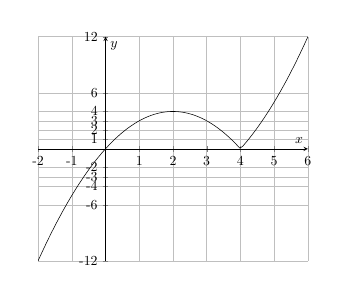
\begin{tikzpicture}[scale=0.5]
\begin{axis}[
    axis lines = middle,
    grid=major,
    legend pos={south west},
    xlabel = {$x$},
    ylabel = {$y$},
    ymin=-12,
    ymax=12,
    xmin=-2,
    xtick={-1,1,3,5,2,-2,4,6},
    xticklabels={-1,1,3,5,2,-2,4,6},
    ytick={ -12,6, 2,-6, -2,1,4,-4,3,-3,12},
    yticklabels={-12, 6, 2,-6, -2,1,4,-4,3,-3,12}           ]
	\addplot[domain=-2:6, samples=100, color=black] {x*abs(4-x)};
%\addplot[domain=-3:5, samples=100, color=black] {-abs(x-1)};
%\addplot[domain=-3.1:2.5, samples=100, color=red] {70*abs(1-2*abs(abs(x)-2))-10*x^2+10*x-70};
	%\addlegendentry{$\text{Рис. 1}$};
\end{axis}
\end{tikzpicture}$$
b) График функции $y=ax-2$ всегда проходит через точку $(0;-2).$ Одну точку пересечения с исходной функцией он имеет только если проходит через точку $(4;0),$ значит  $4a-2=0,\ a=\cfrac{1}{2}.$\\
68. a) $f(x)=x^2-2|x|=\begin{cases}x^2-2x,\ x\geqslant0,\\ x^2+2x,\ x<0.\end{cases}$
$$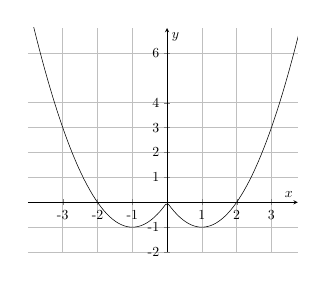
\begin{tikzpicture}[scale=0.5]
\begin{axis}[
    axis lines = middle,
    grid=major,
    legend pos={south west},
    xlabel = {$x$},
    ylabel = {$y$},
    ymin=-2,
    ymax=7,
    xmin=-4,
    xtick={-3,-1,1,3,5,2,-2,4,6},
    xticklabels={-3,-1,1,3,5,2,-2,4,6},
    ytick={ -1,6, 2,-6, -2,1,4,-4,3,-3,12},
    yticklabels={-1, 6, 2,-6, -2,1,4,-4,3,-3,12}           ]
	\addplot[domain=-4:4, samples=100, color=black] {x*x-2*abs(x)};
%\addplot[domain=-3:5, samples=100, color=black] {-abs(x-1)};
%\addplot[domain=-3.1:2.5, samples=100, color=red] {70*abs(1-2*abs(abs(x)-2))-10*x^2+10*x-70};
	%\addlegendentry{$\text{Рис. 1}$};
\end{axis}
\end{tikzpicture}$$
b) Исходя из графика, найдём ответ $a=0.$\\
69. Сумма расстояний от точки $(x;x^2)$ до координатных осей равна $|x|+|x^2|.$ Значит, $|x|+|x^2|=2,\ |x|^2+|x|-2=0,\ (|x|-1)(|x|+2)=0,\ |x|=1,\ x=\pm1,\ y=1.$ Значит, это точки $(-1;1)$ и $(1;1).$\\
70. Построим параболу $y=x^2-4x-5$ по трём точкам $(5;0),\ (-1;0)$ и $(2;-9).$
$$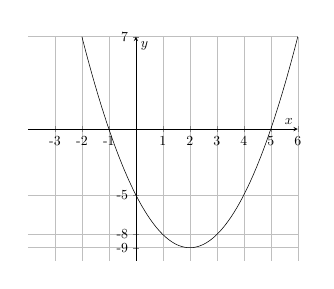
\begin{tikzpicture}[scale=0.5]
\begin{axis}[
    axis lines = middle,
    grid=major,
    legend pos={south west},
    xlabel = {$x$},
    ylabel = {$y$},
    ymin=-10,
    ymax=7,
    xmin=-4,
    xtick={-3,-1,1,3,5,2,-2,4,6},
    xticklabels={-3,-1,1,3,5,2,-2,4,6},
    ytick={ 7, -8, -5,-9},
    yticklabels={7, -8,-5,-9}           ]
	\addplot[domain=-2:6, samples=100, color=black] {x*x-4*x-5};
%\addplot[domain=-3:5, samples=100, color=black] {-abs(x-1)};
%\addplot[domain=-3.1:2.5, samples=100, color=red] {70*abs(1-2*abs(abs(x)-2))-10*x^2+10*x-70};
	%\addlegendentry{$\text{Рис. 1}$};
\end{axis}
\end{tikzpicture}$$
Исходя из графика, наименьшее значение функции на отрезке $[-1;3]$ равно $-9,$ а наибольшее --- 0.\\
71. a) $f(x)=\cfrac{|x^2-x-6|\cdot(x-4)}{3-x}=\cfrac{|x-3|\cdot|x+2|\cdot(x-4)}{3-x}=\begin{cases}-x^2+2x+8,\ x>3,\\ x^2-2x-8,\ x\in[-2;3),\\ -x^2+2x+8,\ x<-2.\end{cases}$
$$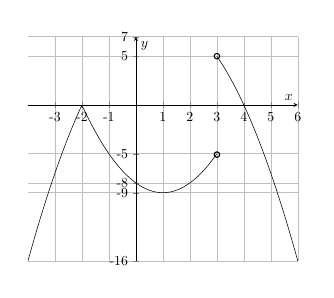
\begin{tikzpicture}[scale=0.5]
\begin{axis}[
    axis lines = middle,
    grid=major,
    legend pos={south west},
    xlabel = {$x$},
    ylabel = {$y$},
    ymin=-16,
    ymax=7,
    xmin=-4,
    xtick={-3,-1,1,3,5,2,-2,4,6},
    xticklabels={-3,-1,1,3,5,2,-2,4,6},
    ytick={ 7, -8, -5,-9,5,-16},
    yticklabels={7, -8,-5,-9,5,-16}           ]
	\addplot[domain=3:6, samples=100, color=black] {(4-x)*(x+2)};
\addplot[domain=-4:3, samples=100, color=black] {abs(x*x-x-6)*(x-4)/(3-x)};
%\addplot[domain=-3:5, samples=100, color=black] {-abs(x-1)};
%\addplot[domain=-3.1:2.5, samples=100, color=red] {70*abs(1-2*abs(abs(x)-2))-10*x^2+10*x-70};
	%\addlegendentry{$\text{Рис. 1}$};
\end{axis}
\draw (4.8,2.7) circle (2pt);
\draw (4.8,5.2) circle (2pt);
\end{tikzpicture}$$
b) Исходя из графика, найдём ответ $p\in(-\infty;-9)\cup(-9;-5)\cup\{0\}\cup[5;+\infty).$\\
72. а) $f(x)=(x+1)|x-1|=\begin{cases}x^2-1,\ x\geqslant1,\\ 1-x^2,\ x<1.\end{cases}$
$$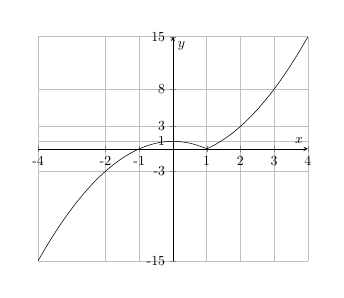
\begin{tikzpicture}[scale=0.5]
\begin{axis}[
    axis lines = middle,
    grid=major,
    legend pos={south west},
    xlabel = {$x$},
    ylabel = {$y$},
    ymin=-15,
    ymax=15,
    xmin=-4,
    xtick={-4,-2,1,4,3,2,-1},
    xticklabels={-4,-2,1,4,3,2,-1},
    ytick={ -15, -3,15,8,1,3},
    yticklabels={-15, -3,15,8,1,3}           ]
	\addplot[domain=-4:4, samples=100, color=black] {(x+1)*abs(x-1)};
%\addplot[domain=-4:3, samples=100, color=black] {abs(x*x-x-6)*(x-4)/(3-x)};
%\addplot[domain=-3:5, samples=100, color=black] {-abs(x-1)};
%\addplot[domain=-3.1:2.5, samples=100, color=red] {70*abs(1-2*abs(abs(x)-2))-10*x^2+10*x-70};
	%\addlegendentry{$\text{Рис. 1}$};
\end{axis}
%\draw (4.8,2.7) circle (2pt);
%\draw (4.8,5.2) circle (2pt);
\end{tikzpicture}$$
б) Исходя из графика, найдём ответ: функция возрастает при $x\in(-\infty;0]$ и $[1;+\infty),$ функция принимает положительные значения при $x\in(-1;1)\cup(1;+\infty),$ уравнение $f(x)=c$ имеет 3 решения при $c\in(0;1).$\\
73. Расстояние от точки $(x;3x^2)$ до прямой $y=x-2$ (то есть $y-x+2=0$) находится по формуле $\rho=\cfrac{|3x^2-x+2|}{\sqrt{1+1}}=2\sqrt{2},\
|3x^2-x+2|=4\Rightarrow \left[\begin{array}{l}3x^2-x+2=4,\\ 3x^2-x+2=-4.\end{array}\right.\Leftrightarrow \left[\begin{array}{l}3x^2-x-2=0,\\ 3x^2-x+6=0.\end{array}\right.\Leftrightarrow\left[\begin{array}{l}x=1,\\ x=-\cfrac{2}{3}.\end{array}\right.$ Значит, это точки
$\left(-\cfrac{2}{3};\cfrac{4}{3}\right)$ и $(1;3).$\\
74. Так как точка $A$ лежит на параболе, $0+0+c=4,\ c=4.$ Так как точка $N$ является вершиной, имеем систему уравнений
$\begin{cases}-\cfrac{b}{2a}=-1,\\ a-b+4=6.\end{cases}\Leftrightarrow\begin{cases}b=2a,\\ b=a-2.\end{cases}\Leftrightarrow\begin{cases}a=-2,\\ b=-4.\end{cases}$\\
75. $y=\sqrt{(1-2x)^2}-3=|2x-1|-3=\begin{cases}2x-4,\ x\geqslant\cfrac{1}{2}\\ -2x-2,\ x<\cfrac{1}{2}.\end{cases}$
$$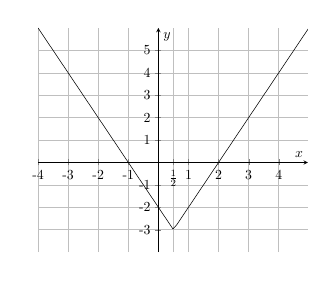
\begin{tikzpicture}[scale=0.5]
\begin{axis}[
    axis lines = middle,
    grid=major,
    legend pos={south west},
    xlabel = {$x$},
    ylabel = {$y$},
    ymin=-4,
    ymax=6,
    xtick={-3, 0.5, -4, -1, 1, 4,3, 6,-2,2,8},
    xticklabels={-3,  $\frac{1}{2}$, -4, -1, 1, 4,3, 6,-2,2,8},
    ytick={-3, -2, 1, -1,3,5,2,4},
    yticklabels={-3, -2, 1, -1,3,5,2,4}            ]
	\addplot[domain=-4:8, samples=100, color=black] {abs(2*x-1)-3};
%\addplot[domain=-3.1:2.5, samples=100, color=red] {70*abs(1-2*abs(abs(x)-2))-10*x^2+10*x-70};
	%\addlegendentry{$\text{Рис. 1}$};
\end{axis}
\end{tikzpicture}$$
Полученный треугольник является равнобедренным, высота, опущенная из его вершины, равна 3, как и основание. Пусть искомый радиус равен $R,$ тогда расстояние от центра окружности до основания равно $3-R$ и по теореме Пифагора $(3-R)^2+\left(\cfrac{3}{2}\right)^2=R^2,\ 9-6R+R^2+\cfrac{9}{4}=R^2,\ R=\cfrac{15}{8}.$\\
76. Раз прямая проходит через начало координат, она задаётся уравнением $y=kx.$ Приравняем прямую к параболе: $kx=(x-1)^2,\ x^2-2x+1-kx=0,\ x^2-(k+2)x+1=0.$ Это уравнение имеет единственное решение при $D=(k+2)^2-4=0,\ k(k+4)=0,\ k=0$ или $k=-4.$ Таким образом, искомые прямые $y=0$ и $y=-4x.$\\
77. Функция $y=bx^2-6x+3$ имеет наименьшее значение при $b>0$ и достигается оно в вершине параболы $x=-\cfrac{-6}{2b}=\cfrac{3}{b}.$ Найдём это значение: $b\cdot\cfrac{9}{b^2}-6\cdot\cfrac{3}{b}+3=3-\cfrac{9}{b}.$ Необходимо, чтобы выполнялось неравенство $3-\cfrac{9}{b}<2,5\Rightarrow\cfrac{9}{b}>0,5
\Rightarrow b<18.$ Значит, $b\in(0;18).$\\
78. Ось $Oy$ пересекается при $x=0,$ значит $0+0+c=-10,\ c=-10.$ Наименьшее значение $a$ соответствует значение в вершине $x=-3,$ которое равно $9-18-10=-19.$\\
79. $\cfrac{x^2+y-2}{x+3}=0\Leftrightarrow\begin{cases}y=2-x^2,\\ x\neq-3.\end{cases}$
$$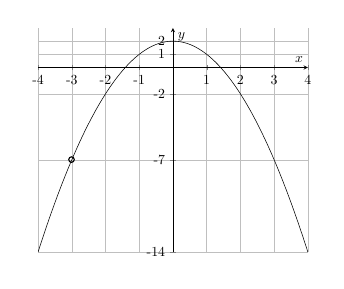
\begin{tikzpicture}[scale=0.5]
\begin{axis}[
    axis lines = middle,
    grid=major,
    legend pos={south west},
    xlabel = {$x$},
    ylabel = {$y$},
    ymin=-14,
    ymax=3,
    xtick={-3, -4, -1, 1, 4,3, 6,-2,2,8},
    xticklabels={-3, -4, -1, 1, 4,3, 6,-2,2,8},
    ytick={-14,-7,-2,1,2},
    yticklabels={-14,-7,-2,1,2}            ]
	\addplot[domain=-4:4, samples=100, color=black] {2-x*x};
%\addplot[domain=-3.1:2.5, samples=100, color=red] {70*abs(1-2*abs(abs(x)-2))-10*x^2+10*x-70};
	%\addlegendentry{$\text{Рис. 1}$};
\end{axis}
\draw (0.85,2.35) circle (2pt);
\end{tikzpicture}$$
Равноудалены от осей координат те точки, у которых $|y|=|x|,$ то есть $|2-x^2|=|x|\Leftrightarrow$\\$\left[\begin{array}{l} 2-x^2=x,\\ 2-x^2=-x.\end{array}\right.
\Leftrightarrow\left[\begin{array}{l} x^2+x-2=0,\\ x^2-x-2=0.\end{array}\right.\Leftrightarrow\left[\begin{array}{l} (x+2)(x-1)=0,\\ (x-2)(x+1)=0.\end{array}\right.$ Значит, это точки $(-2;-2),(2;-2),$\\$(-1;1),(1;1).$\\
80. $$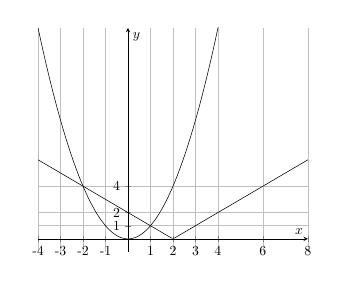
\begin{tikzpicture}[scale=0.5]
\begin{axis}[
    axis lines = middle,
    grid=major,
    legend pos={south west},
    xlabel = {$x$},
    ylabel = {$y$},
    ymin=-1,
    ymax=16,
    xtick={-3, -4, -1, 1, 4,3, 6,-2,2,8},
    xticklabels={-3, -4, -1, 1, 4,3, 6,-2,2,8},
    ytick={-14,-7,-2,1,2,4},
    yticklabels={-14,-7,-2,1,2,4}            ]
	\addplot[domain=-4:8, samples=100, color=black] {x*x};
\addplot[domain=-4:8, samples=100, color=black] {abs(x-2)};
%\addplot[domain=-3.1:2.5, samples=100, color=red] {70*abs(1-2*abs(abs(x)-2))-10*x^2+10*x-70};
	%\addlegendentry{$\text{Рис. 1}$};
\end{axis}
%\draw (0.85,2.35) circle (2pt);
\end{tikzpicture}$$
С осями эти графики пересекаются в точках $(0;0)$ и $(2;0),$ а между собой --- в точках $(-2;4)$ и $(1;1).$\\
81. Приравняем прямую и параболу: $ax-4=ax^2-ax,\ ax^2-2ax+4=0.$ Графики не пересекаются, когда у этого уравнения нет решений. В первом случае при $a=0$ оно вырождается в уравнение $4=0,$ у которого нет корней. Во втором случае $D=4a^2-16a<0,\ a(a-4)<0,\ a\in(0;4).$ Значит, $a\in[0;4).$\\
82. $y=\cfrac{|x-1|}{x-1}(x^2-4)=\begin{cases}x^2-4,\ x>1\\ 4-x^2,\ x<1.\end{cases}$
$$\begin{tikzpicture}[scale=0.5]
\begin{axis}[
    axis lines = middle,
    grid=major,
    legend pos={south west},
    xlabel = {$x$},
    ylabel = {$y$},
    ymin=-6,
    ymax=21,
    xtick={-3,-1,1,3,4},
    xticklabels={-3,-1,1,3,4},
    ytick={-5,-3, 3,5,12},
    yticklabels={-5,-3, 3,5,12}            ]
	\addplot[domain=-4:1, samples=100, color=black] {4-x*x};
\addplot[domain=1:6, samples=100, color=black] {x*x-4};
%\addplot[domain=-3.1:2.5, samples=100, color=red] {70*abs(1-2*abs(abs(x)-2))-10*x^2+10*x-70};
	%\addlegendentry{$\text{Рис. 1}$};
\end{axis}
\draw (3.47,1.89) circle (2pt);
\draw (3.47,0.63) circle (2pt);
\end{tikzpicture}$$
83. $y=\left|\cfrac{2-x}{4}\right|=\begin{cases}\cfrac{x-2}{4},\ x\geqslant2\\ \cfrac{2-x}{4},\ x<2.\end{cases}$
$$\begin{tikzpicture}[scale=0.5]
\begin{axis}[
    axis lines = middle,
    grid=major,
    legend pos={south west},
    xlabel = {$x$},
    ylabel = {$y$},
    ymin=-1,
    ymax=2,
    xtick={-2,-1,2,5,6},
    xticklabels={-2,-1,2,5,6},
    ytick={0.75, 1},
    yticklabels={$\frac{3}{4}$, 1}            ]
	\addplot[domain=-3:7, samples=100, color=black] {abs((2-x)/4)};
%\addplot[domain=1:6, samples=100, color=black] {x*x-4};
%\addplot[domain=-3.1:2.5, samples=100, color=red] {70*abs(1-2*abs(abs(x)-2))-10*x^2+10*x-70};
	%\addlegendentry{$\text{Рис. 1}$};
\end{axis}
%\draw (3.47,1.89) circle (2pt);
%\draw (3.47,0.63) circle (2pt);
\end{tikzpicture}$$
Исходя из графика, найдём ответ $x\in(-2;6).$\\
84. $y=\left|\cfrac{3+x}{6}\right|=\begin{cases}\cfrac{x+3}{6},\ x\geqslant-3\\ \cfrac{-x-3}{6},\ x<-3.\end{cases}$
$$\begin{tikzpicture}[scale=0.5]
\begin{axis}[
    axis lines = middle,
    grid=major,
    legend pos={south west},
    xlabel = {$x$},
    ylabel = {$y$},
    ymin=-1,
    ymax=3,
    xtick={-15,-9,-3,3,9},
    xticklabels={-15,-9,-3,3,9},
    ytick={1,2},
    yticklabels={1,2}            ]
	\addplot[domain=-16:10, samples=100, color=black] {abs((3+x)/6)};
%\addplot[domain=1:6, samples=100, color=black] {x*x-4};
%\addplot[domain=-3.1:2.5, samples=100, color=red] {70*abs(1-2*abs(abs(x)-2))-10*x^2+10*x-70};
	%\addlegendentry{$\text{Рис. 1}$};
\end{axis}
%\draw (3.47,1.89) circle (2pt);
%\draw (3.47,0.63) circle (2pt);
\end{tikzpicture}$$
Исходя из графика, найдём ответ $x\in[-15;9].$\\
85. Пусть парабола задана уравнением $y=ax^2+bx+c.$ Так как в точке $A(0;-3)$ находится вершина, $-\cfrac{b}{2a}=0,\ b=0,\ 0+0+c=-3,\ c=-3.$ Так как парабола проходит через точку $B(6;15),$ имеем уравнение $36a-3=15, a=\cfrac{1}{2}.$ Найдём точки пересечения с осью $Ox:\ \cfrac{1}{2}x^2-3=0,\ x^2=6,\ x=\pm\sqrt{6}.$ Значит, это точки $(-\sqrt{6};0)$ и $(\sqrt{6};0)$\\
86. Пусть парабола задана уравнением $y=ax^2+bx+c.$ Так как в точке $C(0;5)$ находится вершина, $-\cfrac{b}{2a}=0,\ b=0,\ 0+0+c=5,\ c=5.$ Так как парабола проходит через точку $B(4;-3),$ имеем уравнение $16a+5=-3, a=-\cfrac{1}{2}.$ Найдём точки пересечения с осью $Ox:\ -\cfrac{1}{2}x^2+5=0,\ x^2=10,\ x=\pm\sqrt{10}.$ Значит, это точки $(-\sqrt{10};0)$ и $(\sqrt{10};0)$\\
87. Приравняем прямую и параболу: $k=x^2-2x+239,\ x^2-2x+239-k=0.$ Они имеют одну точку пересечения, если получившееся уравнение имеет один корень, поэтому $D=4-4(239-k)=0,\ 239-k=1,\ k=238.$\\
88. Приравняем прямую и параболу: $k=x^2+2x-239,\ x^2+2x-239-k=0.$ Они имеют одну точку пересечения, если получившееся уравнение имеет один корень, поэтому $D=4+4(239+k)=0,\ 239+k=-1,\ k=-240.$\\
89. Это прямоугольный треугольник, вершинами которого являются точки $(0;0),\ \left(\cfrac{1}{2};0\right),\ (0;-1).$ Его катеты равны $\cfrac{1}{2}$ и 1, а значит площадь равна $\cfrac{1}{2}\cdot\cfrac{1}{2}\cdot1=\cfrac{1}{4}.$\\
90. Это прямоугольный треугольник, вершинами которого являются точки $(0;0),\ \left(\cfrac{1}{2};0\right),\ (0;1).$ Его катеты равны $\cfrac{1}{2}$ и 1, а значит площадь равна $\cfrac{1}{2}\cdot\cfrac{1}{2}\cdot1=\cfrac{1}{4}.$\\
91. Это расстояние --- высота, проведённая из прямого угла $AOB$ треугольника с вершинами в точках $A(0;2),\ O(0;0),\ B(1;0).$ Для её нахождения посчитаем площадь этого треугольника двумя способами: $S_{\Delta AOB}=\cfrac{AO\cdot OB}{2}=\cfrac{h\cdot AB}{2},\ 2=h\cdot\sqrt{1^2+2^2},\ h=\cfrac{2\sqrt{5}}{5}.$\\
92. Это расстояние --- высота, проведённая из прямого угла $AOB$ треугольника с вершинами в точках $A(0;2),\ O(0;0),\ B(-1;0).$ Для её нахождения посчитаем площадь этого треугольника двумя способами: $S_{\Delta AOB}=\cfrac{AO\cdot OB}{2}=\cfrac{h\cdot AB}{2},\ 2=h\cdot\sqrt{1^2+2^2},\ h=\cfrac{2\sqrt{5}}{5}.$\\
93. $y=\cfrac{|x^2-5x+6|}{x-2}=\cfrac{|x-2||x-3|}{x-2}=\begin{cases} |x-3|, x>2,\\ -|x-3|, x<2.\end{cases}=\begin{cases} x-3,\ x\geqslant 3,\\ 3-x,\ 2<x<3,\\ x-3,\ x<2.\end{cases}$
$$\begin{tikzpicture}[scale=0.5]
\begin{axis}[
    axis lines = middle,
    grid=major,
    legend pos={south west},
    xlabel = {$x$},
    ylabel = {$y$},
    ymin=-8,
    ymax=8,
    xtick={-3,1,2, 3,6,7},
    xticklabels={-3,1,$ $, 3,6,7},
    ytick={-6,-3,-1,1, 3,4,5},
    yticklabels={-6,-3,-1,1, 3,4,5}            ]
\addplot[domain=-4:2, samples=100, color=black] {-abs(x-3)};
\addplot[domain=2:8, samples=100, color=black] {abs(x-3)};
%\addplot[domain=-3.1:2.5, samples=100, color=red] {70*abs(1-2*abs(abs(x)-2))-10*x^2+10*x-70};
	%\addlegendentry{$\text{Рис. 1}$};
\end{axis}
\draw (3.44,3.185) circle (2pt);
\draw (3.44,2.5) circle (2pt);
\end{tikzpicture}$$
94. $y=\cfrac{|x^2-6x+8|}{x-2}=\cfrac{|x-2||x-4|}{x-2}=\begin{cases} |x-4|, x>2,\\ -|x-4|, x<2.\end{cases}=\begin{cases} x-4,\ x\geqslant 4,\\ 4-x,\ 2<x<4,\\ x-4,\ x<2.\end{cases}$
$$\begin{tikzpicture}[scale=0.5]
\begin{axis}[
    axis lines = middle,
    grid=major,
    legend pos={south west},
    xlabel = {$x$},
    ylabel = {$y$},
    ymin=-8,
    ymax=8,
    xtick={-3,1,2, 3,4,6,7},
    xticklabels={-3,1,2, 3,4,6,7},
    ytick={-7,-3,-2,1,2, 3,4},
    yticklabels={-7,-3,-2,1,2, 3,4}            ]
\addplot[domain=-4:2, samples=100, color=black] {-abs(x-4)};
\addplot[domain=2:8, samples=100, color=black] {abs(x-4)};
%\addplot[domain=-3.1:2.5, samples=100, color=red] {70*abs(1-2*abs(abs(x)-2))-10*x^2+10*x-70};
	%\addlegendentry{$\text{Рис. 1}$};
\end{axis}
\draw (3.44,3.55) circle (2pt);
\draw (3.44,2.15) circle (2pt);
\end{tikzpicture}$$\\
95. $\cfrac{(x-1)(y-3)(y-2x)}{x-2}=0\Leftrightarrow \begin{cases}\left[\begin{array}{l}x=1,\\ y=3,\\ y=2x.\end{array}\right.\\ x\neq2.\end{cases}$
$$\begin{tikzpicture}[scale=0.3]
\tikzset {line01/.style={line width =0.5pt}}
\tikzset{line02/.style={line width =1pt}}
\tikzset{line03/.style={dashed,line width =0.5pt}}
%\filldraw [black] (0,0) circle (1pt);
\draw [->] (-6,0) -- (6,0);
\draw [->] (0,-8) -- (0,10);
\draw[line01] (-3.5,-7) -- (4.5,9);
\draw[line01] (1,-7) -- (1,7);
\draw[line01] (-5,3) -- (5,3);
\draw[line03] (2,0) -- (2,4);
\draw[line03] (0,4) -- (2,4);
%\draw[line03] (0,-2) -- (1,-2);
\draw (6.2,0.7) node {\scriptsize $x$};
%\draw (-1.2,-2) node {\scriptsize $-2$};
%\draw (-0.7,2) node {\scriptsize $2$};
%\draw (-0.7,1.2) node {\scriptsize $1$};
\draw (-1,4) node {\tiny $4$};
\draw (-0.7,2.3) node {\scriptsize $3$};
\draw (2,-0.7) node {\scriptsize $2$};
\draw (0.5,-0.9) node {\tiny $1$};
\draw (0.7,10.2) node {\scriptsize $y$};
\draw (2,4) circle (8pt);
\draw (2,3) circle (8pt);
%\draw (-2,-3) circle (8pt);
\end{tikzpicture}$$
96. $\cfrac{(x-2)(y-1)(y-2x)}{x-1}=0\Leftrightarrow \begin{cases}\left[\begin{array}{l}x=2,\\ y=1,\\ y=2x.\end{array}\right.\\ x\neq1.\end{cases}$
$$\begin{tikzpicture}[scale=0.3]
\tikzset {line01/.style={line width =0.5pt}}
\tikzset{line02/.style={line width =1pt}}
\tikzset{line03/.style={dashed,line width =0.5pt}}
%\filldraw [black] (0,0) circle (1pt);
\draw [->] (-6,0) -- (6,0);
\draw [->] (0,-8) -- (0,10);
\draw[line01] (-3.5,-7) -- (4.5,9);
\draw[line01] (2,-7) -- (2,7);
\draw[line01] (-5,1) -- (5,1);
\draw[line03] (1,0) -- (1,2);
\draw[line03] (0,2) -- (1,2);
%\draw[line03] (0,-2) -- (1,-2);
\draw (6.2,0.7) node {\scriptsize $x$};
%\draw (-1.2,-2) node {\scriptsize $-2$};
%\draw (-0.7,2) node {\scriptsize $2$};
%\draw (-0.7,1.2) node {\scriptsize $1$};
\draw (-1,0.5) node {\tiny $1$};
\draw (-0.7,2.1) node {\scriptsize $2$};
\draw (2.45,-0.7) node {\scriptsize $2$};
\draw (1,-0.9) node {\tiny $1$};
\draw (0.7,10.2) node {\scriptsize $y$};
\draw (1,2) circle (8pt);
\draw (1,1) circle (8pt);
%\draw (-2,-3) circle (8pt);
\end{tikzpicture}$$
97. Пусть парабола задана уравнением $y=ax^2+bx+c.$ Тогда имеем систему $\begin{cases} 5=4a-2b+c,\\ -\cfrac{b}{2a}=-1,\\ 2=a-b+c.\end{cases}\Leftrightarrow
\begin{cases} c=5,\\ b=2a,\\ -a+c=2.\end{cases}\Leftrightarrow \begin{cases} c=5,\\ b=6,\\ a=3.\end{cases}$ Таким образом, парабола задана уравнением $y=3x^2+6x+5.$\\
98. Пусть парабола задана уравнением $y=ax^2+bx+c.$ Тогда имеем систему $\begin{cases} 6=a-b+c,\\ -\cfrac{b}{2a}=1,\\ 2=a+b+c.\end{cases}\Leftrightarrow
\begin{cases} 3a+c=6,\\ b=-2a,\\ -a+c=2.\end{cases}\Leftrightarrow \begin{cases} a=1,\\ b=-2,\\ c=3.\end{cases}$ Таким образом, парабола задана уравнением $y=x^2-2x+3.$\\
99. а) Пусть парабола задана уравнением $y=ax^2+bx+c,$ тогда имеем систему уравнений\\ $\begin{cases} 3=a+b+c,\\ 0=4a+2b+c,\\ 0=a-b+c.\end{cases}
\Leftrightarrow \begin{cases} c=3-a-b,\\ 3a+b+3=0,\\ 3-2b=0.\end{cases}
\Leftrightarrow \begin{cases} c=3,\\ a=-\cfrac{3}{2},\\ b=\cfrac{3}{2}.\end{cases}\Rightarrow y=-\cfrac{3}{2}x^2+\cfrac{3}{2}x+3.$\\
б) Пусть парабола задана уравнением $y=ax^2+bx+c,$ тогда имеем систему уравнений\\ $\begin{cases} 1=a+b+c,\\ 4=4a+2b+c,\\ 11=9a+3b+c.\end{cases}
\Leftrightarrow \begin{cases} c=1-a-b,\\ 3a+b=3,\\ 8a+2b=10.\end{cases}
\Leftrightarrow \begin{cases} c=1-a-b,\\ 3a+b=3,\\ 2a=4.\end{cases}
\Leftrightarrow \begin{cases} c=2\\ b=-3,\\ a=2.\end{cases}
\Rightarrow y=2x^2-3x+2,$ на графике этой квадратичной функции все три точки лежат.\\
100. а) Пусть парабола задана уравнением $y=ax^2+bx+c,$ тогда имеем систему уравнений\\ $\begin{cases} 3=a-b+c,\\ 0=4a-2b+c,\\ 0=a+b+c.\end{cases}
\Leftrightarrow \begin{cases} c=3-a+b,\\ 3a-b+3=0,\\ 3+2b=0.\end{cases}
\Leftrightarrow \begin{cases} c=3,\\ a=-\cfrac{3}{2},\\ b=-\cfrac{3}{2}.\end{cases}\Rightarrow y=-\cfrac{3}{2}x^2-\cfrac{3}{2}x+3.$\\
б) Пусть парабола задана уравнением $y=ax^2+bx+c,$ тогда имеем систему уравнений\\ $\begin{cases} 1=a+b+c,\\ 4=4a+2b+c,\\ 13=9a+3b+c.\end{cases}
\Leftrightarrow \begin{cases} c=1-a-b,\\ 3a+b=3,\\ 8a+2b=12.\end{cases}
\Leftrightarrow \begin{cases} c=1-a-b,\\ 3a+b=3,\\ 2a=6.\end{cases}
\Leftrightarrow \begin{cases} c=4\\ b=-6,\\ a=3.\end{cases}
\Rightarrow y=3x^2-6x+4,$ на графике этой квадратичной функции все три точки лежат.\\
101. До значения $x=-5$ значение функции больше 1. Пусть после $x=-4$ она задана уравнением $y=ax+b,$ тогда имеем систему уравнений $\begin{cases} -4a+b=0,\\ 3a+b=3.\end{cases}\Leftrightarrow \begin{cases} -7a=-3,\\ b=3-3a.\end{cases}\Leftrightarrow \begin{cases} a=\cfrac{3}{7},\\ b=\cfrac{12}{7}.\end{cases}$ Решим неравенство $\cfrac{3}{7}x+\cfrac{12}{7}>1,\ 3x+12>7,\ 3x>-5,\ x>-\cfrac{5}{3}.$ Таким образом, $f(x)>1$ при $x\in(-\infty;-5)\cup\left(-\cfrac{5}{3};+\infty\right).$\\
102. $\cfrac{(y+1)(2x^2-xy-y^2)}{x^2+xy-2y-4}=0\Leftrightarrow \cfrac{(y+1)((x-y)(x+y)+x(x-y))}{(x-2)(x+2)+y(x-2)}=0
\Leftrightarrow \cfrac{(y+1)(x-y)(2x+y)}{(x-2)(x+y+2)}=0\Leftrightarrow\begin{cases}
\left[\begin{array}{l}
y=-1,\\ y=x,\\ y=-2x.\end{array}\right.\\ x\neq2,\\ y\neq-x-2.\end{cases}$
\begin{figure}[ht!]
\center{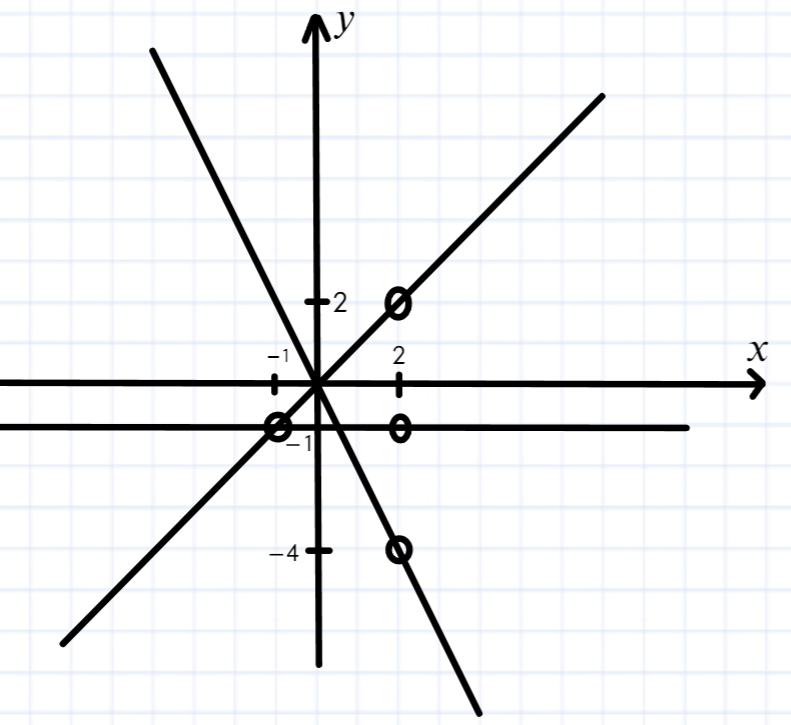
\includegraphics[scale=0.35]{gr8-102.png}}
\end{figure}\\
103.а)$g(x)=\cfrac{4\sqrt{x^2+4x+4}}{\sqrt{16+8x+x^2}+x}=\cfrac{4\sqrt{(x+2)^2}}{\sqrt{(x+4)^2}+x}=\cfrac{4|x+2|}{|x+4|+x}=
\begin{cases} \cfrac{-4(x+2)}{-x-4+x}=x+2,\ x<-4,\\
\cfrac{-4(x+2)}{x+4+x}=-2, -4\leqslant x < -2,\\
\cfrac{4(x+2)}{x+4+x}=2,\ -2<x.\end{cases}$
$$\begin{tikzpicture}[scale=0.3]
\tikzset {line01/.style={line width =0.5pt}}
\tikzset{line02/.style={line width =1pt}}
\tikzset{line03/.style={dashed,line width =0.5pt}}
%\filldraw [black] (0,0) circle (1pt);
\draw [->] (-8,0) -- (6,0);
\draw [->] (0,-8) -- (0,6);
\draw[line01] (-8,-6) -- (-4,-2);
\draw[line01] (-4,-2) -- (-2.3,-2);
\draw[line01] (-1.72,2) -- (6,2);
\draw[line03] (-2,1.8) -- (-2,-1.8);
\draw[line03] (-4,0) -- (-4,-1.8);
\draw[line03] (0,-2) -- (-1.8,-2);
%\draw[line03] (1,0) -- (1,2);
%\draw[line03] (0,2) -- (1,2);
%\draw[line03] (0,-2) -- (1,-2);
\draw (6.2,0.7) node {\scriptsize $x$};
%\draw (-1.2,-2) node {\scriptsize $-2$};
%\draw (-0.7,2) node {\scriptsize $2$};
%\draw (-0.7,1.2) node {\scriptsize $1$};
\draw (-1.7,0.5) node {\tiny $-2$};
\draw (-0.5,2.55) node {\scriptsize $2$};
\draw (-4,0.7) node {\scriptsize $-4$};
\draw (0.6,-2) node {\tiny $-2$};
\draw (0.7,6.2) node {\scriptsize $y$};
\draw (-2,2) circle (8pt);
\draw (-2,-2) circle (8pt);
%\draw (-2,-3) circle (8pt);
\end{tikzpicture}$$
б) Прямая $y=k(x+2)$ при любом значении $k$ проходит через точку $(-2;0).$ При $k=1$ прямая $y=x+2$ совпадает с одной из прямых исходной функции, а значит имеет с данным графиком бесконечное количество точек пересечения. При уменьшении значения $k$ эта прямая пересекает данный график либо только в одной точке (при $x>0$), либо вообще его не пересекает (при $k\leqslant0$). При увеличении значения $k$ прямая будет пересекать данный график в 2 точках (до $x=-2$ и после $x=-2$). Значит, прямая $y=k(x+2)$ имеет с данным графиком более одной общей точки при $k\geqslant1.$\\
104.а) $g(x)=\cfrac{6\sqrt{x^2-2x+1}}{\sqrt{4-4x+x^2}-x}=\cfrac{6\sqrt{(x-1)^2}}{\sqrt{(x-2)^2}-x}=\cfrac{6|x-1|}{|x-2|-x}=
\begin{cases} \cfrac{-6(x-1)}{-x+2-x}=3,\ x<1,\\
\cfrac{6(x-1)}{-x+2-x}=-3,\ 1< x \leqslant 2,\\
\cfrac{6(x-1)}{x-2-x}=3-3x,\ 2<x.\end{cases}$
$$\begin{tikzpicture}[scale=0.3]
\tikzset {line01/.style={line width =0.5pt}}
\tikzset{line02/.style={line width =1pt}}
\tikzset{line03/.style={dashed,line width =0.5pt}}
%\filldraw [black] (0,0) circle (1pt);
\draw [->] (-8,0) -- (6,0);
\draw [->] (0,-8) -- (0,6);
\draw[line01] (2,-3) -- (3,-6);
\draw[line01] (-7,3) -- (0.7,3);
\draw[line01] (1.3,-3) -- (2,-3);
\draw[line03] (1,2.8) -- (1,-2.8);
\draw[line03] (2,0) -- (2,-2.8);
\draw[line03] (0,-3) -- (0.8,-3);
%\draw[line03] (1,0) -- (1,2);
%\draw[line03] (0,2) -- (1,2);
%\draw[line03] (0,-2) -- (1,-2);
\draw (6.2,0.7) node {\scriptsize $x$};
%\draw (-1.2,-2) node {\scriptsize $-2$};
%\draw (-0.7,2) node {\scriptsize $2$};
%\draw (-0.7,1.2) node {\scriptsize $1$};
\draw (1.3,0.5) node {\tiny $1$};
\draw (-0.5,2.55) node {\scriptsize $3$};
\draw (2,0.5) node {\tiny $2$};
\draw (-0.8,-3) node {\tiny $-3$};
\draw (0.7,6.2) node {\scriptsize $y$};
\draw (1,3) circle (8pt);
\draw (1,-3) circle (8pt);
%\draw (-2,-3) circle (8pt);
\end{tikzpicture}$$
б) Прямая $y=k(x-1)$ при любом значении $k$ проходит через точку $(1;0).$ При $k=-3$ прямая $y=3-3x$ совпадает с одной из прямых исходной функции, а значит имеет с данным графиком бесконечное количество точек пересечения. При увеличении значения $k$ эта прямая пересекает данный график либо только в одной точке (при $x<0$), либо вообще его не пересекает (при $k\geqslant0$). При уменьшении значения $k$ прямая будет пересекать данный график в 2 точках (до $x=1$ и после $x=1$). Значит, прямая $y=k(x-1)$ имеет с данным графиком более одной общей точки при $k\leqslant-3.$\\
105. $y=\cfrac{2x(4x^2-1)}{2x^2-x}=\cfrac{2x(2x-1)(2x+1)}{x(2x-1)}=4x+2,\ x\notin\left\{0;\cfrac{1}{2}\right\}.$
$$\begin{tikzpicture}[scale=0.3]
\tikzset {line01/.style={line width =0.5pt}}
\tikzset{line02/.style={line width =1pt}}
\tikzset{line03/.style={dashed,line width =0.5pt}}
%\filldraw [black] (0,0) circle (1pt);
\draw [->] (-4,0) -- (4,0);
\draw [->] (0,-10) -- (0,10);
\draw[line01] (-3,-10) -- (2,10);
\draw[line03] (0.5,0) -- (0.5,3.7);
\draw[line03] (0,4) -- (0.2,4);
%\draw[line03] (1,0) -- (1,2);
%\draw[line03] (0,2) -- (1,2);
%\draw[line03] (0,-2) -- (1,-2);
\draw (4.2,0.7) node {\scriptsize $x$};
%\draw (-1.2,-2) node {\scriptsize $-2$};
%\draw (-0.7,2) node {\scriptsize $2$};
%\draw (-0.7,1.2) node {\scriptsize $1$};
\draw (0.5,-1) node {\tiny $\cfrac{1}{2}$};
\draw (-0.7,2) node {\tiny $2$};
\draw (-0.5,4) node {\tiny $4$};
\draw (0.7,10.2) node {\scriptsize $y$};
\draw (0,2) circle (8pt);
\draw (0.5,4) circle (8pt);
%\draw (-2,-3) circle (8pt);
\end{tikzpicture}$$
$y\in(-\infty;2)\cup(2;4)\cup(4;+\infty).$\\
106. $y=\cfrac{2x(x^2-9)}{x^2-3x}=\cfrac{2x(x-3)(x+3)}{x(x-3)}=2x+6,\ x\notin\left\{0;3\right\}.$
$$\begin{tikzpicture}[scale=0.3]
\tikzset {line01/.style={line width =0.5pt}}
\tikzset{line02/.style={line width =1pt}}
\tikzset{line03/.style={dashed,line width =0.5pt}}
%\filldraw [black] (0,0) circle (1pt);
\draw [->] (-6,0) -- (6,0);
\draw [->] (0,-3) -- (0,14);
\draw[line01] (-4,-2) -- (3.5,13);
\draw[line03] (3,0) -- (3,11.7);
\draw[line03] (0,12) -- (2.7,12);
%\draw[line03] (1,0) -- (1,2);
%\draw[line03] (0,2) -- (1,2);
%\draw[line03] (0,-2) -- (1,-2);
\draw (6.2,0.7) node {\scriptsize $x$};
%\draw (-1.2,-2) node {\scriptsize $-2$};
%\draw (-0.7,2) node {\scriptsize $2$};
%\draw (-0.7,1.2) node {\scriptsize $1$};
\draw (3,-0.5) node {\tiny $3$};
\draw (-0.7,6) node {\tiny $6$};
\draw (-0.7,12) node {\tiny $12$};
\draw (0.7,14.2) node {\scriptsize $y$};
\draw (0,6) circle (8pt);
\draw (3,12) circle (8pt);
%\draw (-2,-3) circle (8pt);
\end{tikzpicture}$$
$y\in(-\infty;6)\cup(6;12)\cup(12;+\infty).$\\
107. $(|x-2|-1)(y+x^2-2x-3)=0\Leftrightarrow\left[\begin{array}{l}|x-2|=1,\\y=-x^2+2x+3.\end{array}\right.\Leftrightarrow
\left[\begin{array}{l}x=3,\\x=1\\y=-x^2+2x+3.\end{array}\right.$
$$\begin{tikzpicture}[scale=0.5]
\tikzset {line01/.style={line width =0.5pt}}
\begin{axis}[
    axis lines = middle,
    grid=major,
    legend pos={south west},
    xlabel = {$x$},
    ylabel = {$y$},
    ymin=-12,
    ymax=5,
    xtick={-2,-1,1, 2, 3,4},
    xticklabels={-2,-1,1,2, 3,4},
    ytick={-5,3, 4},
    yticklabels={-5,3, 4}            ]
\addplot[domain=-3:5, samples=100, color=black] {-x*x+2*x+3};
%\addplot[domain=-3.1:2.5, samples=100, color=red] {70*abs(1-2*abs(abs(x)-2))-10*x^2+10*x-70};
	%\addlegendentry{$\text{Рис. 1}$};
\end{axis}
\draw[line01] (3.4,0) -- (3.4,6);
\draw[line01] (5.15,0) -- (5.15,6);
%\draw (3.44,3.185) circle (2pt);
%\draw (3.44,2.5) circle (2pt);
\end{tikzpicture}$$
108. а) $\cfrac{(x^2+4x+3)(x-1)}{x+1}=\cfrac{(x+1)(x+3)(x-1)}{x+1}=x^2+2x-3,\ x\neq-1.$
$$\begin{tikzpicture}[scale=0.5]
\begin{axis}[
    axis lines = middle,
    grid=major,
    legend pos={south west},
    xlabel = {$x$},
    ylabel = {$y$},
    ymin=-5,
    ymax=13,
    xtick={-5, -3, -2, -1, 1, 3},
    xticklabels={-5, -3, -2, -1, 1, 3},
    ytick={-4, -3,12},
    yticklabels={-4, -3,12}             ]
	\addplot[domain=-6:5, samples=100, color=black] {x*x+2*x-3};
%\addplot[domain=-3.1:2.5, samples=100, color=red] {70*abs(1-2*abs(abs(x)-2))-10*x^2+10*x-70};
	%\addlegendentry{$\text{Рис. 1}$};
\end{axis}
\draw (3.43,0.33) circle (2pt);
\end{tikzpicture}$$
б) По графику определим, что функция принимает значения $(-4;-3].$\\
109. $y=\cfrac{x^2-10x+24}{|x-7|+|x-3|-2}=\begin{cases}
\cfrac{(x-6)(x-4)}{7-x+3-x-2}=\cfrac{6-x}{2},\ x<3,\\
\cfrac{(x-6)(x-4)}{7-x+x-3-2}=\cfrac{x^2-10x+24}{2},\ 3\leqslant x \leqslant 7,\\
\cfrac{(x-6)(x-4)}{x-7+x-3-2}=\cfrac{x-4}{2},\ 7<x.\end{cases}$
$$\begin{tikzpicture}[scale=0.5]
\begin{axis}[
    axis lines = middle,
    grid=major,
    legend pos={south west},
    xlabel = {$x$},
    ylabel = {$y$},
    ymin=-3,
    ymax=7,
    xtick={-4, 3 , 5, 7, 10, 4, 6},
    xticklabels={-4, 3 , 5, 7, 10, 4, 6},
    ytick={ 5, 4,  -0.5, 1.5,3},
    yticklabels={  5, 4,  $-\frac{1}{2}$, 1.5,3}           ]
\addplot[domain=-5:3, samples=100, color=black] {(6-x)/2};
\addplot[domain=3:7, samples=100, color=black] {(x*x-10*x+24)/2};
\addplot[domain=7:11, samples=100, color=black] {(x-4)/2};
%\addplot[domain=-3.1:2.5, samples=100, color=red] {70*abs(1-2*abs(abs(x)-2))-10*x^2+10*x-70};
	%\addlegendentry{$\text{Рис. 1}$};
\end{axis}
\end{tikzpicture}$$
110. $y=\cfrac{x^2-8x+15}{|x-6|+|x-2|-2}=\begin{cases}
\cfrac{(x-5)(x-3)}{6-x+2-x-2}=\cfrac{5-x}{2},\ x<2,\\
\cfrac{(x-5)(x-3)}{6-x+x-2-2}=\cfrac{x^2-8x+15}{2},\ 2\leqslant x \leqslant 6,\\
\cfrac{(x-5)(x-3)}{x-6+x-2-2}=\cfrac{x-3}{2},\ 6<x.\end{cases}$
$$\begin{tikzpicture}[scale=0.5]
\begin{axis}[
    axis lines = middle,
    grid=major,
    legend pos={south west},
    xlabel = {$x$},
    ylabel = {$y$},
    ymin=-3,
    ymax=7,
    xtick={-5, -3 , 1, 2, 3, 5, 6, 9, 4},
    xticklabels={-5, -3 , 1, 2, 3, 5, 6, 9, 4},
    ytick={-0.5, 5, 4, 2, 1.5, 3},
    yticklabels={$-\frac{1}{2}$, 5, 4, 2, 1.5, 3}           ]
\addplot[domain=-6:2, samples=100, color=black] {(5-x)/2};
\addplot[domain=2:6, samples=100, color=black] {(x*x-8*x+15)/2};
\addplot[domain=6:10, samples=100, color=black] {(x-3)/2};
%\addplot[domain=-3.1:2.5, samples=100, color=red] {70*abs(1-2*abs(abs(x)-2))-10*x^2+10*x-70};
	%\addlegendentry{$\text{Рис. 1}$};
\end{axis}
\end{tikzpicture}$$
111. Парабола всегда симметрична относительно вертикальной прямой, проходящей через её вершину, поэтому второй корень равен $\cfrac{7}{2}+\left(\cfrac{7}{2}-\sqrt{2}\right)=7-\sqrt{2}.$\\
112. Парабола всегда симметрична относительно вертикальной прямой, проходящей через её вершину, поэтому второй корень равен $\cfrac{5}{2}+\left(\cfrac{5}{2}-\sqrt{3}\right)=5-\sqrt{2}.$\\
113. Первые две прямые пересекаются в точке $(0;0).$ Найдём точку пересечения первой прямой и третьей: $\begin{cases}y=\cfrac{2}{3}x,\\ x+y=5.\end{cases}
\Leftrightarrow \begin{cases}y=\cfrac{2}{3}x,\\ x+\cfrac{2}{3}x=5.\end{cases}
\Leftrightarrow \begin{cases}y=2,\\ x=3.\end{cases}$ Найдём точку пересечения второй прямой и третьей: $\begin{cases}y=4x,\\ x+y=5.\end{cases}
\Leftrightarrow \begin{cases}y=4x,\\ x+4x=5.\end{cases}
\Leftrightarrow \begin{cases}y=4,\\ x=1.\end{cases}$ Таким образом, искомый треугольник имеет вершины в точках $(0;0),\ (3;2),\ (1;4).$\\
\begin{figure}[ht!]
\center{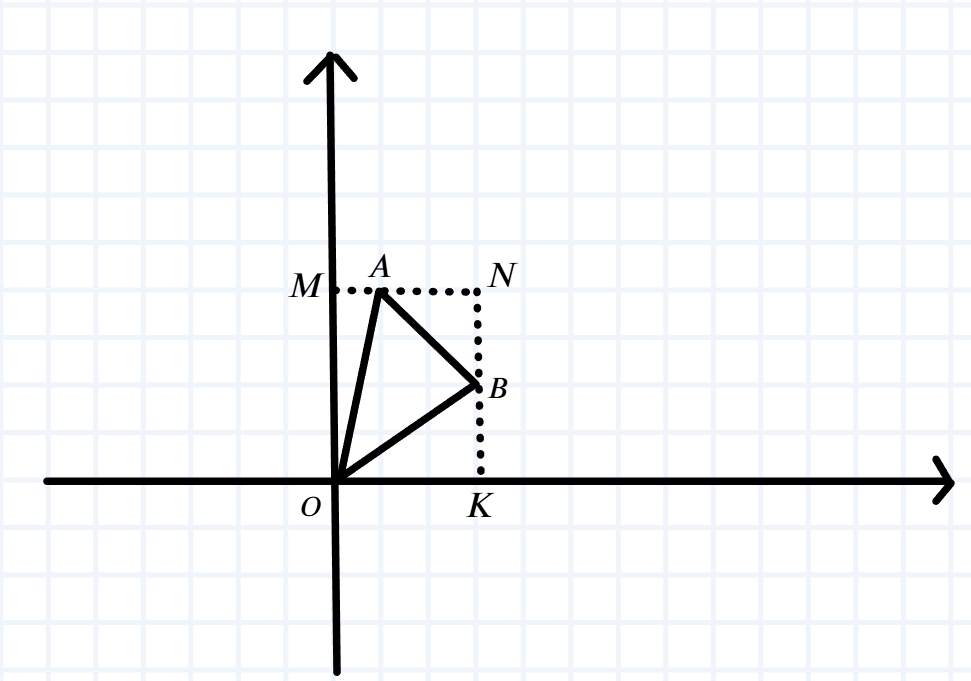
\includegraphics[scale=0.35]{g9-1000.png}}
\end{figure}\\
Достроив треугольник до прямоугольника, найдём его площадь: $S_{\Delta AOB}=S_{OMNK}-S_{\Delta OMA}-S_{\Delta ANB}-S_{\Delta OBK}=
3\cdot4-1\cdot4:2-2\cdot2:2-3\cdot2:2=5.$\\
114. Первые две прямые пересекаются в точке $(0;0).$ Найдём точку пересечения первой прямой и третьей: $\begin{cases}y=\cfrac{4}{3}x,\\ x+y=7.\end{cases}
\Leftrightarrow \begin{cases}y=\cfrac{2}{3}x,\\ x+\cfrac{4}{3}x=7.\end{cases}
\Leftrightarrow \begin{cases}y=4,\\ x=3.\end{cases}$ Найдём точку пересечения второй прямой и третьей: $\begin{cases}y=6x,\\ x+y=7.\end{cases}
\Leftrightarrow \begin{cases}y=6x,\\ x+6x=7.\end{cases}
\Leftrightarrow \begin{cases}y=6,\\ x=1.\end{cases}$ Таким образом, искомый треугольник имеет вершины в точках $(0;0),\ (3;4),\ (1;6).$\\
\begin{figure}[ht!]
\center{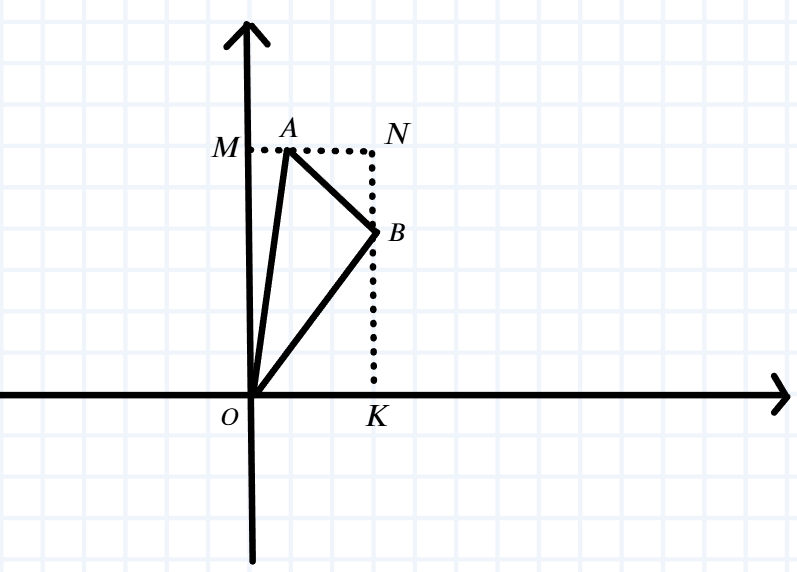
\includegraphics[scale=0.35]{g9-1001.png}}
\end{figure}\\
Достроив треугольник до прямоугольника, найдём его площадь: $S_{\Delta AOB}=S_{OMNK}-S_{\Delta OMA}-S_{\Delta ANB}-S_{\Delta OBK}=
3\cdot6-1\cdot6:2-2\cdot2:2-3\cdot4:2=7.$\\
115. а) $$\begin{tikzpicture}[scale=0.5]
\begin{axis}[
    axis lines = middle,
    grid=major,
    legend pos={south west},
    xlabel = {$x$},
    ylabel = {$y$},
    ymin=-55,
    ymax=5,
    xtick={-6,-4,-2, 2,4,6,10},
    xticklabels={-6,-4,-2, 2,4,6,10},
    ytick={-53,-35,-15,1,-3},
    yticklabels={-53,-35,-15,1,-3}            ]
\addplot[domain=-8:10, samples=100, color=black] {-x*x+4*x-3};
\end{axis}
\end{tikzpicture}$$\\
б) $$\begin{tikzpicture}[scale=0.5]
\begin{axis}[
    axis lines = middle,
    grid=major,
    legend pos={south west},
    xlabel = {$x$},
    ylabel = {$y$},
    ymin=-55,
    ymax=5,
    xtick={-6,-4,-2, 2,4,6,10},
    xticklabels={-6,-4,-2, 2,4,6,10},
    ytick={-53,-35,-15,1,-3},
    yticklabels={-53,-35,-15,1,-3}            ]
\addplot[domain=-10:10, samples=100, color=black] {-x*x+4*abs(x)-3};
\end{axis}
\end{tikzpicture}$$\\
116. а) $$\begin{tikzpicture}[scale=0.5]
\begin{axis}[
    axis lines = middle,
    grid=major,
    legend pos={south west},
    xlabel = {$x$},
    ylabel = {$y$},
    ymin=-55,
    ymax=5,
    xtick={-6,-4, -2,1,4,6,10},
    xticklabels={-6,-4, -2,1,4,6,8},
    ytick={-45,-21,-5,4,-5},
    yticklabels={-45,-21,-5,4,-5}            ]
\addplot[domain=-8:10, samples=100, color=black] {-x*x+2*x+3};
\end{axis}
\end{tikzpicture}$$\\
б) $$\begin{tikzpicture}[scale=0.5]
\begin{axis}[
    axis lines = middle,
    grid=major,
    legend pos={south west},
    xlabel = {$x$},
    ylabel = {$y$},
    ymin=-55,
    ymax=5,
    xtick={-8, -6,-4,-1, 1,4,6,8},
    xticklabels={-8,-6,-4,-1, 1,4,6,8},
    ytick={-45,-21,4},
    yticklabels={-45,-21,4}            ]
\addplot[domain=-10:10, samples=100, color=black] {-x*x+2*abs(x)+3};
\end{axis}
\end{tikzpicture}$$
\newpage
